%%% Hlavní soubor. Zde se definují základní parametry a odkazuje se na ostatní části. %%%

%% Verze pro jednostranný tisk:
% Okraje: levý 40mm, pravý 25mm, horní a dolní 25mm
% (ale pozor, LaTeX si sám přidává 1in)
\documentclass[12pt,a4paper]{report}
\setlength\textwidth{145mm}
\setlength\textheight{247mm}
\setlength\oddsidemargin{15mm}
\setlength\evensidemargin{15mm}
\setlength\topmargin{0mm}
\setlength\headsep{0mm}
\setlength\headheight{0mm}
% \openright zařídí, aby následující text začínal na pravé straně knihy
\let\openright=\clearpage

%% Pokud tiskneme oboustranně:
% \documentclass[12pt,a4paper,twoside,openright]{report}
% \setlength\textwidth{145mm}
% \setlength\textheight{247mm}
% \setlength\oddsidemargin{14.2mm}
% \setlength\evensidemargin{0mm}
% \setlength\topmargin{0mm}
% \setlength\headsep{0mm}
% \setlength\headheight{0mm}
% \let\openright=\cleardoublepage

%% Vytváříme PDF/A-2u
\usepackage[a-2u]{pdfx}

%% Přepneme na českou sazbu a fonty Latin Modern
\usepackage[czech]{babel}
\usepackage{lmodern}
\usepackage[T1]{fontenc}
\usepackage{textcomp}

%% Použité kódování znaků: obvykle latin2, cp1250 nebo utf8:
\usepackage[utf8]{inputenc}

%%% Další užitečné balíčky (jsou součástí běžných distribucí LaTeXu)
\usepackage{amsmath}        % rozšíření pro sazbu matematiky
\usepackage{amsfonts}       % matematické fonty
\usepackage{amsthm}         % sazba vět, definic apod.
\usepackage{bbding}         % balíček s nejrůznějšími symboly
			    % (čtverečky, hvězdičky, tužtičky, nůžtičky, ...)
\usepackage{bm}             % tučné symboly (příkaz \bm)
\usepackage{graphicx}       % vkládání obrázků ------ reduce data usage=======================================================================================================================================================

\usepackage{fancyvrb}       % vylepšené prostředí pro strojové písmo
\usepackage{indentfirst}    % zavede odsazení 1. odstavce kapitoly
\usepackage{natbib}         % zajištuje možnost odkazovat na literaturu
			    % stylem AUTOR (ROK), resp. AUTOR [ČÍSLO]
\usepackage[nottoc]{tocbibind} % zajistí přidání seznamu literatury,
                            % obrázků a tabulek do obsahu
\usepackage{icomma}         % inteligetní čárka v matematickém módu
\usepackage{dcolumn}        % lepší zarovnání sloupců v tabulkách
\usepackage{booktabs}       % lepší vodorovné linky v tabulkách
\usepackage{paralist}       % lepší enumerate a itemize
\usepackage{xcolor}         % barevná sazba

 % vlastni pridavky--------------------------------------------------------
\usepackage{microtype}
\usepackage{hyphenat}
\usepackage[section]{placeins} %obrazky zustavaji ve stejne sekci


%%% Údaje o práci

% Název práce v jazyce práce (přesně podle zadání)
\def\NazevPrace{Vizualizace dostupnosti veřejnou dopravou}

% Název práce v angličtině
\def\NazevPraceEN{Travel Times Visualization Based on Public Transport Timetable}

% Jméno autora
\def\AutorPrace{Jan Fürst}

% Rok odevzdání
\def\RokOdevzdani{2022}

% Název katedry nebo ústavu, kde byla práce oficiálně zadána
% (dle Organizační struktury MFF UK, případně plný název pracoviště mimo MFF)
\def\Katedra{Katedra teoretické informatiky a matematické logiky}
\def\KatedraEN{Department of Theoretical Computer Science and Mathematical Logic}

% Jedná se o katedru (department) nebo o ústav (institute)?
\def\TypPracoviste{Katedra}
\def\TypPracovisteEN{Department}

% Vedoucí práce: Jméno a příjmení s~tituly
\def\Vedouci{Mgr. Martin Pilát, Ph.D.}

% Pracoviště vedoucího (opět dle Organizační struktury MFF)
\def\KatedraVedouciho{Katedra teoretické informatiky a matematické logiky}
\def\KatedraVedoucihoEN{Department of Theoretical Computer Science and Mathematical Logic}

% Studijní program a obor
\def\StudijniProgram{Informatika}
\def\StudijniObor{Programování a softwarové systémy}

% Nepovinné poděkování (vedoucímu práce, konzultantovi, tomu, kdo
% zapůjčil software, literaturu apod.)
\def\Podekovani{%
Rád bych poděkoval panu Mgr. Martinu Pilátovi, Ph.D. za cenné rady při vedení mé práce. Dále bych rád poděkoval členům své rodiny za podporu během psaní bakalářské práce.
}

% Abstrakt (doporučený rozsah cca 80-200 slov; nejedná se o zadání práce)
\def\Abstrakt{
% problem - popis kontextu problemu
Mnoho lidí jezdí denně veřejnou dopravou a~mnohým z~nich by pomohlo, kdyby bydleli na místě ze kterého se dopraví rychleji na jimi často navštěvovaná místa. Problém však je, jak takové místo k~bydlení najít.
% nase reseni + hlavni prinos
To řešíme v~naší webové aplikaci, ve které zobecňujeme klasické vyhledávání cest v~jízdních řádech a~umožňujeme tak vyhodnocovat dostupnost z~uživatelem zadaných míst na všechna ostatní místa. Pro snadné vyhledávání vizualizujeme, na všech dostupných místech, vypočtenou dostupnost v~interaktivní mapě.
% (mozna) abstrakce zaveru: komu by se to mohlo hodit
Naše webová aplikace pracuje s~interní knihovnou, která zpřístupňuje funkcionalitu potřebnou pro vyhodnocení dostupnosti. Tuto knihovnu lze využít samostatně a~řešit tak jiné problémy, které vyžadují vyhodnocení dostupnosti veřejnou dopravou.
}
\def\AbstraktEN{
%problem
People often use public transport to travel to places they visit on regular basis. For these people, it would be very useful if they could live in a~place, from which they could get faster to all the places they visit. The problem is how to find such a~place.
%our solution
This problem is what we are trying to solve in our web application. By generalizing the standard public transport search we make it possible to calculate the travel times from user-defined places to all other reachable places. We visualize calculated travel times in an interactive map to simplify the search for the suitable place with the lowest travel times.
%usefulnes
Our web application uses our internal library which contains the functionality required for travel time calculations. This library could be used independently on the web application to solve other problems that require evaluation of travel times by public transport.
}

% 3 až 5 klíčových slov (doporučeno), každé uzavřeno ve složených závorkách
\def\KlicovaSlova{%
{GTFS}, {RAPTOR}, {Vizualizace dostupnosti}
}
\def\KlicovaSlovaEN{%
{GTFS}, {RAPTOR}, {Travel Times Visualization}
}

%% Balíček hyperref, kterým jdou vyrábět klikací odkazy v PDF,
%% ale hlavně ho používáme k uložení metadat do PDF (včetně obsahu).
%% Většinu nastavítek přednastaví balíček pdfx.
\hypersetup{unicode}
\hypersetup{breaklinks=true}

%% Definice různých užitečných maker (viz popis uvnitř souboru)
%%% Tento soubor obsahuje definice různých užitečných maker a prostředí %%%
%%% Další makra připisujte sem, ať nepřekáží v ostatních souborech.     %%%

%%% Drobné úpravy stylu

% Tato makra přesvědčují mírně ošklivým trikem LaTeX, aby hlavičky kapitol
% sázel příčetněji a nevynechával nad nimi spoustu místa. Směle ignorujte.
\makeatletter
\def\@makechapterhead#1{
  {\parindent \z@ \raggedright \normalfont
   \Huge\bfseries \thechapter. #1
   \par\nobreak
   \vskip 20\p@
}}
\def\@makeschapterhead#1{
  {\parindent \z@ \raggedright \normalfont
   \Huge\bfseries #1
   \par\nobreak
   \vskip 20\p@
}}
\makeatother

% Toto makro definuje kapitolu, která není očíslovaná, ale je uvedena v obsahu.
\def\chapwithtoc#1{
\chapter*{#1}
\addcontentsline{toc}{chapter}{#1}
}

% Trochu volnější nastavení dělení slov, než je default.
\lefthyphenmin=2
\righthyphenmin=2

% Zapne černé "slimáky" na koncích řádků, které přetekly, abychom si
% jich lépe všimli.
\overfullrule=1mm

%%% Makra pro definice, věty, tvrzení, příklady, ... (vyžaduje baliček amsthm)

\theoremstyle{plain}
\newtheorem{veta}{Věta}
\newtheorem{lemma}[veta]{Lemma}
\newtheorem{tvrz}[veta]{Tvrzení}

\theoremstyle{plain}
\newtheorem{definice}{Definice}

\theoremstyle{remark}
\newtheorem*{dusl}{Důsledek}
\newtheorem*{pozn}{Poznámka}
\newtheorem*{prikl}{Příklad}

%%% Prostředí pro důkazy

\newenvironment{dukaz}{
  \par\medskip\noindent
  \textit{Důkaz}.
}{
\newline
\rightline{$\qedsymbol$}
}

%%% Prostředí pro sazbu kódu, případně vstupu/výstupu počítačových
%%% programů. (Vyžaduje balíček fancyvrb -- fancy verbatim.)

\DefineVerbatimEnvironment{code}{Verbatim}{fontsize=\small, frame=single}

%%% Prostor reálných, resp. přirozených čísel
\newcommand{\R}{\mathbb{R}}
\newcommand{\N}{\mathbb{N}}

%%% Užitečné operátory pro statistiku a pravděpodobnost
\DeclareMathOperator{\pr}{\textsf{P}}
\DeclareMathOperator{\E}{\textsf{E}\,}
\DeclareMathOperator{\var}{\textrm{var}}
\DeclareMathOperator{\sd}{\textrm{sd}}

%%% Příkaz pro transpozici vektoru/matice
\newcommand{\T}[1]{#1^\top}

%%% Vychytávky pro matematiku
\newcommand{\goto}{\rightarrow}
\newcommand{\gotop}{\stackrel{P}{\longrightarrow}}
\newcommand{\maon}[1]{o(n^{#1})}
\newcommand{\abs}[1]{\left|{#1}\right|}
\newcommand{\dint}{\int_0^\tau\!\!\int_0^\tau}
\newcommand{\isqr}[1]{\frac{1}{\sqrt{#1}}}

%%% Vychytávky pro tabulky
\newcommand{\pulrad}[1]{\raisebox{1.5ex}[0pt]{#1}}
\newcommand{\mc}[1]{\multicolumn{1}{c}{#1}}


%% Titulní strana a různé povinné informační strany
\begin{document}
%%% Titulní strana práce a další povinné informační strany

%%% Titulní strana práce

\pagestyle{empty}
\hypersetup{pageanchor=false}

\begin{center}

\centerline{\mbox{
\includegraphics[width=166mm]{../img/logo-cs.pdf}}}

\vspace{-8mm}
\vfill

{\bf\Large BAKALÁŘSKÁ PRÁCE}

\vfill

{\LARGE\AutorPrace}

\vspace{15mm}

{\LARGE\bfseries\NazevPrace}

\vfill

\Katedra

\vfill

{
\centerline{\vbox{\halign{\hbox to 0.45\hsize{\hfil #}&\hskip 0.5em\parbox[t]{0.45\hsize}{\raggedright #}\cr
Vedoucí bakalářské práce:&\Vedouci \cr
\noalign{\vspace{2mm}}
Studijní program:&\StudijniProgram \cr
\noalign{\vspace{2mm}}
Studijní obor:&\StudijniObor \cr
}}}}

\vfill

% Zde doplňte rok
Praha \RokOdevzdani

\end{center}

\newpage

%%% Následuje vevázaný list -- kopie podepsaného "Zadání bakalářské práce".
%%% Toto zadání NENÍ součástí elektronické verze práce, nescanovat.

%%% Strana s čestným prohlášením k bakalářské práci

\openright
\hypersetup{pageanchor=true}
\pagestyle{plain}
\pagenumbering{roman}
\vglue 0pt plus 1fill

\noindent
Prohlašuji, že jsem tuto bakalářskou práci vypracoval(a) samostatně a výhradně
s~použitím citovaných pramenů, literatury a dalších odborných zdrojů.
Tato práce nebyla využita k získání jiného nebo stejného titulu.

\medskip\noindent
Beru na~vědomí, že se na moji práci vztahují práva a povinnosti vyplývající
ze zákona č. 121/2000 Sb., autorského zákona v~platném znění, zejména skutečnost,
že Univerzita Karlova má právo na~uzavření licenční smlouvy o~užití této
práce jako školního díla podle §60 odst. 1 autorského zákona.

\vspace{10mm}

\hbox{\hbox to 0.5\hsize{%
V \hbox to 6em{\dotfill} dne \hbox to 6em{\dotfill}
\hss}\hbox to 0.5\hsize{\dotfill\quad}}
\smallskip
\hbox{\hbox to 0.5\hsize{}\hbox to 0.5\hsize{\hfil Podpis autora\hfil}}

\vspace{20mm}
\newpage

%%% Poděkování

\openright

\noindent
\Podekovani

\newpage

%%% Povinná informační strana bakalářské práce

\openright

\vbox to 0.5\vsize{
\setlength\parindent{0mm}
\setlength\parskip{5mm}

Název práce:
\NazevPrace

Autor:
\AutorPrace

\TypPracoviste:
\Katedra

Vedoucí bakalářské práce:
\Vedouci, \KatedraVedouciho

Abstrakt:
\Abstrakt

Klíčová slova:
\KlicovaSlova

\vss}\nobreak\vbox to 0.49\vsize{
\setlength\parindent{0mm}
\setlength\parskip{5mm}

Title:
\NazevPraceEN

Author:
\AutorPrace

\TypPracovisteEN:
\KatedraEN

Supervisor:
\Vedouci, \KatedraVedoucihoEN

Abstract:
\AbstraktEN

Keywords:
\KlicovaSlovaEN

\vss}

\newpage

\openright
\pagestyle{plain}
\pagenumbering{arabic}
\setcounter{page}{1}


%%% Strana s automaticky generovaným obsahem bakalářské práce

\tableofcontents

%%% Jednotlivé kapitoly práce jsou pro přehlednost uloženy v samostatných souborech

\chapter*{Úvod}
\addcontentsline{toc}{chapter}{Úvod}

% popis kontextu
Každý by chtěl bydlet v~blízkosti míst, která často navštěvuje. V~dnešní době se však většina těchto míst nachází ve větších městech kde jsou ceny bydlení vyšší. Ne každý má dostatek finančních prostředků k~tomu, aby mohl bydlet v~blízkosti navštěvovaných míst. Mnozí, zejména ti kteří cestují hromadou dopravou, pak tráví dennodenně dlouhé hodiny na cestách.

Lidé navíc často navštěvují různorodá místa, jako jsou třeba zaměstnání, škola, známí, lékaři či různé obchody. Ani pro člověka s~dostatkem finančních prostředků tedy nemusí být snadné naleznout ideální lokalitu, odkud by byl schopen dostat se na často navštěvovaná místa v~minimálním čase.

% podobne prace
V~současné době existuje mnoho způsobů, jak nalézt optimální cestu hromadnou dopravou mezi dvěma místy. Pokud vím, není k~dispozici vyhledávač, který by tento koncept rozšiřoval a~byl schopen nalézt optimální cesty mezi několika zadanými a~všemi ostatními místy.

% cile prace
Na základě tohoto rozšířeného konceptu se v~této práci pokusíme ohodnotit všechna místa podle dostupnosti veřejnou dopravou ze zadaných míst v~daných časech. Vypočtenou dostupnost vizualizujeme ve všech místech a~tím umožníme snadnou orientaci ve výsledcích. Pro zpřístupnění aplikace běžným uživatelům vytvoříme webovou aplikaci. Výsledky aplikace budou pro uživatele dopočteny v~přijatelném čase. Samotná aplikace bude dostatečně obecná, aby byla schopna pracovat s~jízdními řády z~různých lokalit.

% popis jednotlivych kapitol
V~první kapitole detailně popisujeme cíle práce.
Ve~druhé kapitole popisujeme data jízdních řádů a~jejich poskytovatele.
Ve třetí kapitole popisujeme námi zvolený algoritmus pro hledání cest v~jízdních řádech.
Ve čtvrté kapitole popisujeme vlastní úpravy algoritmu zvoleného v~předchozí kapitole.
V~páté kapitole zobecňujeme algoritmus z~předchozí kapitoly a~umožňujeme tak vyhledávat dostupnost z~několika vstupních míst na všechna ostatní výstupní místa.
V šesté kapitole popisujeme přístupy k~vizualizaci dostupnosti.
V~sedmé kapitole popisujeme implementaci myšlenek, popsaných v~předchozích kapitolách a~popisujeme také implementaci webové aplikace.
V~osmé kapitole si ukážeme, jak naše aplikace funguje s~jízdními řády z~různých lokalitách.
V~příloze dokumentujeme, jak se má naše aplikace zprovoznit a~jak ji lze nakonfigurovat.

% nepopisuji zaver - nevim jak moc je takovy popis potreba 

\chapter{Cíle práce}

V~této kapitole si detailně popíšeme cíle, kterých se budeme snažit dosáhnout. Zbylé kapitoly budou řešit některé z~cílů uvedených zde.

\section{Terminologie}\label{data-terminologie}

\begin{itemize}
    \item \textbf{Dostupnost} definujeme jako dobu, za jakou se ze vstupního místa dostaneme na cílové místo. S~takto definovanou dostupností se nám, v~porovnání s~konkrétními časy, bude snáze pracovat ve statistických výpočtech.\label{definice-dostupnosti}
    
    \item \textbf{Místo} je nějaká pozice v~prostoru, která není příliš vzdálená od některé ze zastávek. V~této práci zásadně odlišujeme význam místa a~zastávky.

    \item \textbf{Zastávka} je místo, na kterém staví nějaký spoj.

    \item \textbf{Trip} překládáme jako \textbf{jízdu}. Jízda je posloupnost zastávek.
    
    \item \textbf{Route} překládáme jako \textbf{trasu}. Trasa je množina jízd jedoucích přes stejné zastávky.
    
    V~kapitole~\ref{kapitola-1} však pracujeme s~\textbf{GTFS trasou}, jejíž definice se liší od definice trasy, kterou používáme v~následujících kapitolách. GTFS trasy totiž mohou obsahovat jízdy, které jedou přes různé množiny zastávek.
    
    \item \textbf{Transfers} překládáme jako \textbf{přestupy}. Přestupovat můžeme mezi dvěma zastávkami a~přestup trvá nějaký čas.
    
    \item \textbf{Spoj} používáme pro nějaký dopravní prostředek, který jede v~konkrétní čas po zastávkách jízdy. %podobnost s TripWithDate v impl.
    
    \item \textbf{Journey} překládáme jako cestu. Cesta je posloupnost spojů a~přestupů, kterými se dopravíme z~počátečního místa na cílové.

\end{itemize}


\section{Požadavky na aplikaci}
% trosku to souvisi s implementaci ze sekce 5.4 kde aplikaci popisuju - i kdyz tam ale popisuju existujici design

\subsubsection{Frontend by měl:}
\begin{itemize}
    \item Poskytovat rozhraní pro zadávání vstupu uživatelem.
    
    Uživatel může zadávat více často navštěvovaných míst.
    
    Zadané místo musí být v~dostatečné blízkosti nějaké zastávky.
    
    S~místem lze asociovat důležitost, která určuje, jak moc je dostupnost z~tohoto místa zohledněna ve vypočtených dostupnostech.
    
    Uživatel může s~jedním místem asociovat více časů, ve kterých chce z~místa odjíždět.
    
    Uživatel má mít možnost nezadávat čas přesně, ale nechat aplikaci vyhodnotit dostupnost pro nějaké okolí zadaného času.
    
    \item Poskytovat rozhraní pro zobrazování výstupu uživateli.
    
    Na výstupu se uživateli vizualizuje vypočtená dostupnost.
    
    Dostupnost má být vizualizovaná na všech místech.
    
    Uživatel má být ve vizualizaci schopen snadno najít dostupnost pro konkrétní místa.
    
    \item Posílat požadavky na backend, který běží na serveru.
\end{itemize}

\subsubsection{Backend by měl:}
\begin{itemize}
    \item Zpracovávat dotazy z~frontendu v~rozumném čase. % maximálně jednotky sekund
    
    \item Aktualizovat data jízdních řádů.
    
    \item Delegovat vyhodnocení dostupnosti na knihovnu.
\end{itemize}

\subsubsection{Knihovna by měla:} %sjednoceni s backendem ???
\begin{itemize}
    \item Být nezávislá na webové aplikaci.
    
    \item Dostatečně obecná, aby mohla pracovat s~jízdními řády po celém světě.
    
    \item Načítat data jízdních řádů a~přetransformovat je do formátu vhodného pro vyhledávání.
    
    \item Pro daný vstup vyhodnocovat dostupnost na všech místech. % klicova cast prace
\end{itemize}


\section{Problémy k~řešení}


\subsubsection{Data}\label{problemyKReseni-data}

Nejprve potřebujeme mít přístup k~datům jízdních řádů. Bez samotných dat se nemůžeme pokoušet vyhodnocovat dostupnost.


\subsubsection{Vyhodnocení dostupnosti}\label{problemyKReseni-dostupnost}

Pro vyhodnocení dostupnosti musíme nejprve nalézt cesty, které vedou mezi vstupními a~výstupními místy. Tento problém si rozdělíme na následující podproblémy, které budeme postupně řešit.

\begin{itemize}
    \item Vyhledání cesty mezi 2 zastávkami. To je klasický problém, který řeší běžné vyhledávače.
    
    \item Vyhledání cesty mezi 1 vstupní zastávkou a~všemi ostatními zastávkami. Toto je důležité, neboť cílíme na vyhodnocení dostupnosti na všech místech. Vyhodnocení dostupnosti na všech zastávkách je tedy přirozený mezikrok.
    
    \item Zadávání více vstupních zastávek. Vstupní zastávky jsou ty, které uživatel zadává jako často navštěvovaná místa. Takových zastávek je, v~porovnání se všemi zastávkami, velmi málo. Tento mezikrok potřebujeme, abychom uživatelům umožnili zadávat více často navštěvovaných míst.
    
    \item Zobecnění cílové zastávky na místo. V~této fázi jsme již schopni vyhodnocovat dostupnost na všech zastávkách. Abychom byli schopni vyhodnocovat dostupnost na libovolných místech, potřebujeme zobecnit zastávky na místa.
    
    \item Zobecnění vstupní zastávky na místo. Toto zobecnění potřebujeme, neboť chceme našim uživatelům umožnit zadávat na vstupu libovolná místa, ne jen zastávky.
    
    \item Vyhledávání oběma směry. Předchozí podproblémy počítají se situací, kdy uživatelem zadaná místa jsou ta, ze kterých chce vyjíždět. Uživatele by však mohla zajímat situace, kdy na zadaná místa chce v~daný čas přijíždět. Tuto možnost mají některé vyhledávače, které umožňují vyhledávat spoje dle času dojezdu.
    
    \item Vyhodnocování dostupnosti pro časový interval. Vyřešení tohoto podproblému by umožnilo uživatelům nezadávat vstupní čas přesně. Mohli bychom totiž vyhodnocovat dostupnost pro nějaké okolí zadaného času.
\end{itemize}


\subsubsection{Vizualizace}\label{problemyKReseni-vizualizace}

Potřebujeme zajistit způsob vizualizace, který uživatelům umožní dohledat ideální místo podle dostupnosti.

Potřebujeme najít způsob, jak vizualizovat dostupnost pro všechna místa.

% usnadnili orientaci ve výsledcích a~umožnili jim snadné vyhledávání nejdostupnějších míst



% chybi prestupy? ---- to vsak zalezi i na datech, v tuhle chvili to tedy nejspise neni problem

% v dalsich kapitolach se chci odkazovat na pozadavky, ktere prave resim

\chapter{Data jízdních řádů}\label{kapitola-1}

V~této kapitole řešíme naši potřebu přístupu k~datům, zmíněnou jíž v~sekci~\ref{problemyKReseni-data}.

Tato data jsou dostupná v~různých datových formátech, v~České republice například ve formátu JDF (Jednotný datový formát). Tento a~jemu podobné proprietární formáty však sdílí stejnou nevýhodu. Aplikace pracující s~nimi buď nejsou schopny pracovat s~daty od jiných zprostředkovatelů, nebo musí vytvářet netriviální adaptéry. Takový přístup je zcela nepřípustný, zvláště existují-li alternativy.

Vhodnou alternativou je formát GTFS \citep{gtfs}. Tento formát je spravovaný společností Google a~je ve světě v~podstatě standardem pro popis jízdních řádů.

\section{Zdroje dat}

Za účely vývoje aplikace je vhodné pracovat s~daty, která nám jsou co možná nejbližší, proto budeme pracovat s~daty jízdních řádů v~České republice. Taková data, ve vhodném formátu GTFS \citep{gtfs}, poskytuje společnost Pražské integrované dopravy \citet{pidData}.

Dalším zdrojem dat, nejen pro Českou republiku, je \url{https://transitfeeds.com/}. Vůbec největším zdrojem jednotných dat, se kterými budeme pracovat jsou GTFS for Germany, dostupné na \url{https://gtfs.de/en/feeds/de\_nv/}.

\section{GTFS}\label{gtfs-popis}

Formát GTFS je rozšířením formátu CSV (Comma-separated values). GTFS nevynucuje typ dat, nedá se tedy spoléhat na to, že např. \textbf{id} budou uložena jako čísla. Všechna data z~formátu GTFS, relevantní pro náš problém, jsou zobrazena na obrázku~\ref{fig:gtfs-data}.

\begin{figure}[ht]
    \centering
    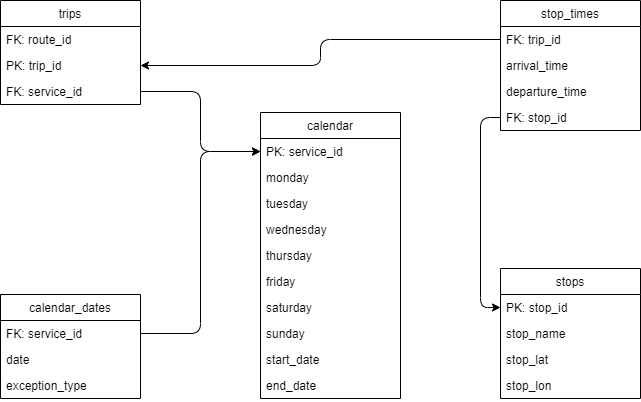
\includegraphics[width=0.75\textwidth]{../img/gtfs-data}
    \caption{Relevantní obsah souborů ve formátu GTFS.}
    \label{fig:gtfs-data}
\end{figure}

Následuje krátký popis nejdůležitějších rysů každé z~používaných složek.
\begin{itemize}
    \item Soubor stops.txt obsahuje geografické souřadnice ve formátu WGS84 (World Geodetic System), ty použijeme k~vizualizaci a~ke generování přestupů. Formát GTFS sice obsahuje přestupy v~transfers.txt, ty však obsahují jen oficiální přestupy, ne všechny možné.
    
    Mezi zastávkami mohou existovat takové zastávky, na kterých nestaví žádný spoj. Takové zastávky budeme chtít odstranit.
    
    \item Soubor stop\_times.txt obsahuje informace o~příjezdu a~odjezdu z~jednotlivých zastávek. Dle specifikace formátu GTFS, může časový formát příjezdů a~odjezdů přesahovat klasický 24 hodinový formát. Taková situace nastává u~spojů, které jedou souvisle přes půlnoc.

    \item \textbf{Route\_id} ze souboru trips.txt identifikuje GTFS trasu, pod kterou patří skupina jízd. 
    
    \textbf{Route\_id} společně se všemi zastávkami, přes které trasa jede, použijeme k~identifikaci pozměněného významu trasy, který používáme v~následujících kapitolách.
    
    \item Soubor calendar.txt přiřazuje k~jízdě dny, kdy je provozována. Každý řádek v~kalendáři má navíc omezenou platnost. Podle GTFS best practices, popsaných na adrese \url{https://gtfs.org/schedule/best-practices/}, by měla být minimální platnost nejméně 7 dnů.

    \item V~souboru calendar\_dates.txt jsou explicitně vypsány výjimky, kdy je jízda provozována a~podle kalendáře by být neměla, nebo naopak kdy jízda není provozována a~podle kalendáře by být měla.
\end{itemize}
\chapter{Hledání cest}\label{kapitola-2}

V~této kapitole řešíme problém hledání cesty mezi dvěma zastávkami, který jsme popsali již v~sekci~\ref{problemyKReseni-dostupnost}.

Pro vyhledávání cest v~jízdních řádech potřebujeme nějaký algoritmus. Existující řešení spadají v~zásadě do dvou kategorií.

\begin{enumerate}
    \item Algoritmy řešící problém jako grafový. Hledání nejkratších cest v~jízdních řádech však není snadná úloha, neboť cestovat hromadnou dopravou se dá jen ve chvíli, kdy jede nějaký spoj. Existující přístupy pak musí řešit problém čekání na zastávce. Důsledkem toho je obecně pomalejší hledání.

    \item Algoritmy neřešící problém jako grafový. Jedním z~hlavních zástupců této kategorie je algoritmus RAPTOR \citet{raptor}. Tento algoritmus nevyžaduje předzpracovaná data, každou trasu navštíví maximálně jednou a~dá se počítat paralelně. Navíc umožňuje omezit počet přestupů během výpočtu.
\end{enumerate}

\section{RAPTOR}

\subsection{Data}\label{raptor-data}

RAPTOR bude pracovat s~daty z~formátu GTFS. Nejprve je však musíme převést do datové struktury, která bude podporovat operace vyžadované algoritmem RAPTOR.

Pro každou trasu si potřebujeme pamatovat zastávky, přes které trasa vede, uspořádané od první po poslední. Dále si chceme zapamatovat také jízdy, které jedou po trase, uspořádané od nejdřívější k~nejpozdější.

Pro každou zastávku si uložíme všechny trasy, na kterých zastávka leží. Ke každé zastávce přiřazujeme \textbf{multilabel}, který pro každou iteraci obsahuje nejdřívější čas příjezdu.

Dále si potřebujeme uložit přestupy, které musí být tranzitivní. Ty však nejsou součástí GTFS dat a~budeme si je tedy muset vygenerovat. Generování přestupů konkrétně popíšeme v~sekci~\ref{generovani-prestupu}.

Budeme si chtít ukládat také seznam označených zastávek. Ten slouží k~optimálnějšímu procházení tras.

\subsection{Popis algoritmu}\label{raptor-popisAlgo}

RAPTOR je založený na metodě dynamického programování, pracuje tedy v~iteracích. Aktuální iteraci označujeme indexem $k$.

Vstupem je počáteční zastávka, čas výjezdu a~cílová zastávka.

Výstupem je cesta s~minimálním časem dojezdu skládající se z~maximálně $k$~jízd a~$k-1$~přestupů.

Při výpočtu každé iterace dodržujeme invariant, že na začátku $k$-té~iterace jsou hodnoty \textbf{multilabelu} do indexu~$k-1$ správné.

Začínáme inicializací. Nejdřívější časy příjezdu v~\textbf{multilabelu} každé zastávky nastavíme na nekonečno. Počáteční zastávku přidáme do seznamu označených zastávek. \textbf{Multilabel} v~nulté iteraci nastavíme na čas výjezdu ze vstupu. Aktuální iteraci nastavíme na~1.

Dále pro každou iteraci provádíme následující tři fáze.
\begin{enumerate}
    \item V~první fázi propagujeme, v~rámci všech \textbf{multilabelů}, příjezdové časy z~předchozí iterace do aktuální iterace. Tím nastavíme horní mez pro příjezd v~této iteraci.
    
    Dále projdeme označené zastávky a~uložíme si množinu označených tras, které obsahují označenou zastávku. Pro každou označenou trasu si navíc pamatujeme zastávku skrze kterou byla trasa označena. Pokud označujeme již označenou trasu, zapamatujeme si tu zastávku, která leží blíže začátku trasy.
    
    Vyprázdníme seznam označených zastávek, abychom v~následující iteraci procházeli jen nově označené zastávky.
    
    \begin{code}
foreach stop:
  stop.multilabel[k] = stop.multilabel[k-1]

  foreach markedStop in markedStops:
    foreach route in markedStop.Routes:
      markedRoutes.addOrUpdate(route, markedStop)
  
  markedStops.clear()
    \end{code}
    
    \item Ve druhé fázi projdeme všechny označené trasy.
    
    Postupně procházíme zastávky na trase, od první označené, dokud nenarazíme na zastávku pro kterou máme definovanou nejdřívější jízdu. Jednodušeji řečeno, hledáme jízdu na kterou můžeme přestoupit, neboli jízdu, ve které z~aktuální zastávky odjíždíme poději, než na ni přijedeme v~$k-1$~iteraci.
    
    Následně projdeme všechny zbylé zastávky a~pokusíme se aktualizovat čas příjezdu na tyto zastávky s~využitím právě nalezené nejdřívější jízdy.
    
    Mohlo se nám však stát, že jsme v~$k-1$~iteraci přijeli na některou ze zastávek dříve, než kdy na ni přijedeme aktuálně nejdřívější jízdou. Z~takové zastávky se musíme znovu pokusit nalézt nejdřívější jízdu.

    \begin{code}
foreach (route, markedStop) in markedRoutes:
  # find earliest trip
  foreach stop on route (in order) beginning from markedStop:
    foreach trip on route (in order):
        if(stop.multilabel[k-1] < trip.departureTimeFrom(stop)):
          currentStop = stop
          currentTrip = trip
          break

    foreach stop on route (in order) beginning from currentStop:
      currentTrip = tryFindEarliestTripThan(currentTrip)
      stop.updateMultilabelByTrip(currentTrip) #marks updated
    \end{code}

    \item Ve třetí fázi využijeme přestupy z~nově označených zastávek. Každým přestupem se pokusíme aktualizovat čas příjezdu na zastávku, na kterou přestupujeme.
    
    \begin{code}
foreach markedStop:
  foreach transfer from markedStop:
    transfer.targetStop.updateMultilabelByTransfer()#marks updated
    \end{code}
\end{enumerate}

Aktualizací času myslíme zápis příjezdového času do \textbf{multilabelu} pro $k$-tou~iteraci. Při úspěšné aktualizaci příjezdového času na zastávku ve druhé a~třetí fází zastávku označujeme.

Algoritmus se zastaví v~případě, že dosáhl omezení počtu iterací, nebo pokud v~první fází neexistují žádné označené zastávky, tedy není co vylepšovat.


\subsection{Zrychlení algoritmu}

\subsubsection{Optimalizace}\label{raptor-optimalizace}

RAPTOR popsaný v~\citet{raptor} navíc využívá optimalizace \textbf{lokální prořezávání} a~\textbf{cílové prořezávání}.

\begin{itemize}
    \item Optimalizace \textbf{lokálního prořezávání} zavádí navíc pro každou zastávku položku, jenž obsahuje dosavadní nejdřívější čas příjezdu. Díky této optimalizaci nemusíme v~první fázi algoritmu propagovat příjezdové časy. K~zápisu příjezdových časů do \textbf{multilabelu} tedy dochází jen ve chvíli, kdy časy aktualizujeme. Vypozorovali jsme, že tato optimalizace vede ke zhruba $5\%$ zrychlení vyhledávání.
    
    \item Optimalizace \textbf{cílového prořezávání} spočívá v~tom, že neoznačujeme zastávky s~příjezdovým časem vyšším než je aktuální příjezdový čas na cílové zastávce.
\end{itemize}

\subsubsection{Paralelizace}\label{raptor-paralelizace}

Algoritmus je možné zrychlit paralelizací viz \citet[Sekce 3.3]{raptor}. Konkrétně se jedná o~paralelizaci druhé fáze algoritmu, která je časově nejnáročnější.
\chapter{Úpravy algoritmu RAPTOR}
%pouzivam `RAPTORa` ale jinde jsem se toho spise zbavil ...
%mozna bych mel prekontrolovat - upravoval jsem

V~této kapitole si popíšeme, jak jsme upravili algoritmus RAPTOR popsaný v~kapitole~\ref{kapitola-2}.

Následující úpravy nám pomohou řešit problémy, související s~vyhodnocováním dostupnosti, popsané v~sekci~\ref{problemyKReseni-dostupnost}.

Vyřešíme problém:
\begin{itemize}
    \item Vyhledání cesty mezi 1 vstupní zastávkou a~všemi ostatními zastávkami
\end{itemize}

Navrhneme řešení problému:
\begin{itemize}
    \item Vyhledávání oběma směry.
\end{itemize}


\section{Námi provedené úpravy}

\subsubsection{Zrušení cílového prořezávání}

Optimalizace cílového prořezávání, popsaná v~sekci~\ref{raptor-optimalizace}, je vhodná, pokud hledáme pouze dobu příjezdu na cílovou zastávku. Pokud ale tuto optimalizaci nevyužijeme a~neurčíme dokonce ani cílovou zastávku, pak můžeme tento algoritmus využít k~výpočtu příjezdového času na všechny dostupné zastávky.

\subsubsection{Spouštění algoritmu z~více počátečních zastávek} \label{raptor-vicePocatecnichZastavek}

Pro zobecnění vstupní zastávky na místo budeme potřebovat vypočítat časy příjezdu ze zastávek v~okolí zadaného místa na všechny cílové zastávky. Toto zobecnění detailně popisujeme v~sekci~\ref{zobecneni-zadavaniMista}.

Opakované spouštění algoritmu RAPTOR je velice neefektivní. Naštěstí se dá tento problém řešit mnohem jednodušeji úpravou algoritmu.

Místo jedné počáteční zastávky spustíme RAPTORa na několika počátečních zastávkách. Počátečními zastávkami myslíme zastávky v~okolí zadaného místa. V~inicializaci označíme všechny počáteční zastávky a~každé zastávce nastavíme hodnotu \textbf{multilabelu} v~nulté iteraci na součet vstupního času a~času potřebnému k~příchodu na zastávku ze zadaného místa.

\subsubsection{Hledání cest v~intervalu} \label{raptor-interval}
%velka cast je z RAPTORa - nema byt v predchozi sekci

Pro statisticky přesnější výpočty dostupnosti bychom chtěli spouštět RAPTORa opakovaně v~určitém intervalu. Opakované spouštění RAPTORa však vede k~násobnému zpomalení výpočtu. Řešením je upravená verze rRAPTOR detailně popsaná v~\citet[Sekce 4.2]{raptor}.

Nevýhodou tohoto řešení je, že v~něm nemůžeme využít optimalizace lokálního prořezávání, popsaného v~sekci~\ref{raptor-optimalizace}. Použití položky s~dosavadním nejdřívějším příjezdem by vedlo ke ztrátě významu hodnot \textbf{multilabelu} v~jednotlivých iteracích, nemohli bychom tedy omezeným počtem iterací omezit počet přestupů. Navíc bychom tím porušili invariant.

V~upravené verzi rRAPTOR spouštíme algoritmus postupně od posledního času v~intervalu k~prvnímu. Mezi jednotlivými spuštěními však zachováme hodnoty \textbf{multilabelu}. Navíc v~první fázi algoritmu smíme povolit jen propagaci příjezdových časů, které jsou dřívější, než příjezdové časy nastavené v~aktuální iteraci.

Co je velice důležité a~v~původním článku není popsané, je vyhodnocování nejdřívějšího času příjezdu na zastávku. Jelikož se výpočty intervalu mohou lišit v~počtu iterací, není jasné, ve které iteraci se uchovává celkově nejdřívější čas příjezdu. Při vyhodnocování tedy musíme projít příjezdové časy \textbf{multilabelu} pro všechny iterace a~nejmenší z~časů je námi hledaným ohodnocením.

Tato upravená verze vede ke zrychlení celkového výpočtu časů z~intervalu. Míra zrychlení závisí na časových odstupech v~intervalu a~na hustotě jízd. Pro hrubou představu jsme se při výpočtech dvou časů v~intervalu pěti minut dostali ze 2-násobného na zhruba 1,1-násobné zpomalení celkového času výpočtu.


\section{Vyhledávání oběma směry}

Chtěli bychom, aby vypočtená dostupnost na zastávkách byla symetrická. Tím myslíme to, že by měla být vypočtena nejen z~času, za který se ze zadaného místa dostaneme na cílové místo, ale i~z~času, za který se z~cílového místa dostaneme na zadané místo.

Jízdní řády se zdají být poměrně symetrické. Mohlo by se tedy zdát, že opačný směr můžeme zanedbat. Není to však pravidlem.

Jednoduchá záměna počátečního a~cílového místa není možná, neboť počátečních míst je mnohem méně než cílových míst. Následně by algoritmus RAPTOR musel počítat dostupnost z~každého cílového místa na všechna ostatní místa a~to není možné vypočítat v~rozumném čase.

Tento problém bychom však mohli vyřešit inverzí chodu algoritmu RAPTOR.

\subsubsection{\uv{Inverze} chodu algoritmu}\label{raptor-inverze}

RAPTOR umí počítat jen s~časem výjezdu z~počáteční zastávky. Pokud bychom chtěli počítat s~časem dojezdu na cílovou zastávku, mohli bychom využít inverze chodu algoritmu.

Inverze chodu je zde použita ve smyslu obrácení významu času. Takový RAPTOR by cestoval proti směru jízd a~hledal by navazující jízdy, které jedou dříve, než je zastávka navštívena.


\chapter{Zobecnění Vyhledávání}\label{kapitola-3}

V~této kapitole vyřešíme zbylé problémy s~vyhodnocováním dostupnosti ze sekce~\ref{problemyKReseni-dostupnost}:
\begin{itemize}
    \item Zobecnění vstupní zastávky na místo.

    \item Zobecnění cílové zastávky na místo.

    \item Zadávání více vstupních zastávek.
    
    \item Vyhodnocování dostupnosti pro časový interval.
\end{itemize}


\section{Zobecnění vstupní zastávky na místo}\label{zobecneni-zadavaniMista}

Pro zobecnění vstupní zastávky na místo potřebujeme vypočítat dostupnost ze všech zastávek v~okolí vstupního místa na všechny dostupné zastávky. Zastávky v~okolí vstupního místa jsou ty, na které jsme schopni přijít pěšky a~odjet z~nich nějakým spojem.

Dostupnost ze vstupního místa na cílovou zastávku je rovna součtu doby strávené chůzí na zastávku v~okolí, času, kdy čekáme na příjezd spoje, a~doby jízdy z~této zastávky na cílovou zastávku. Pro každou cílovou zastávku navíc bereme právě minimální dostupnost ze všech dostupností vypočtených ze zastávek v~okolí vstupního místa.

Problém však je, že zastávek v~okolí vstupního místa může být mnoho a~následné spouštění algoritmu RAPTOR z~každé této zastávky je velice výpočetně náročné.

Dále popíšeme naše přístupy k~optimalizaci výpočtu.

\subsubsection{Výběr $k$-nejbližších sousedů}

Výběrem $k$-nejbližších sousedů snížíme počet sousedních zastávek a~tím urychlíme výpočet.

Pro místa s~velkou hustotou zastávek však mohou být výsledky velice nepřesné, neboť zanedbáváme velké množství zastávek, které sice nepatří mezi nejbližší, ale jsme schopni na ně dojít pěšky.

Navíc nevyužíváme vlastnosti, že přes blízko položené zastávky často jezdí stejné spoje.

\subsubsection{Rozdělení zastávek do ekvivalenčních tříd}

Definujeme relaci ekvivalence pro zastávky dle spojů, které přes tyto zastávky jezdí. Do stejné ekvivalenční třídy tedy umístíme všechny zastávky, přes které jezdí stejné spoje.

Dále z~každé ekvivalenční třídy vybereme jednoho reprezentanta, např. takovou zastávku, která je nejblíže k~zadanému místu.

Seznam všech reprezentantů tvoří zastávky v~okolí, ze kterých nám stačí spouštět výpočet.

Toto řešení sice eliminuje některé zastávky, ukázalo se však, že výsledný počet zastávek je stále příliš vysoký.

\subsubsection{(Minimální) pokrytí množiny}

V~tomto přístupu máme množinu zastávek z~okolí zadané zastávky a~chceme najít podmnožinu této množiny takovou, že sjednocení všech spojů jedoucích přes zastávky množin budou ekvivalentní.

Tento problém lze řešit výpočtem minimálního pokrytí množiny. To je sice NP-úplný problém, my si však vystačíme s~aproximačním algoritmem, který tento problém řeší v~polynomiálním čase.

Výsledky tohoto přístupu jsou lepší než ty, ke kterým vedly předchozí přístupy. Algoritmus RAPTOR je však stále spouštěn pro každou zastávku zvlášť, přestože trasy které algoritmem procházíme se značně překrývají.

\subsubsection{RAPTOR spuštěn s~více počátečními zastávkami}\label{raptor-zobecneni-vicePocatecnichZastavek}

Úprava, popsaná v~kapitole~\ref{raptor-vicePocatecnichZastavek}, nám umožňuje označit za počáteční zastávky všechny zastávky z~okolí zadaného místa.

To znamená, že si vystačíme s~jediným spuštěním algoritmu RAPTOR a~bez znatelného zpomalení běhu algoritmu.


\section{Zobecnění cílové zastávky na místo}\label{zobecneni-ciloveZastavkyNaMista}

Vyhledávání příjezdového času z~jednoho zadaného místa na libovolné místo, které je v~pěší vzdálenosti od dostupných zastávek, lze řešit minimálně následujícími dvěma způsoby.

\subsubsection{Rozdělení mapy na segmenty}

Mapu rozdělíme na segmenty. Pro každý segment určíme zastávku ze které aproximujeme, v~závislosti na rychlosti chůze, dojezdové časy do ostatních míst v~segmentu.

Pokud bychom zvolili segmenty stejné velikosti, měli bychom buď příliš mnoho segmentů, nebo by výpočty pro lokality s~velkou hustotou zastávek nebyly příliš přesné. Ideální by tedy bylo mít segmenty různě velké, v~závislosti na hustotě zastávek.

Tento přístup se zdá být z~pohledu implementace poměrně složitý, navíc aproximace v~rámci segmentu nemusí dávat dostatečně přesné výsledky.

\subsubsection{Využití zastávek z~okolí}

Tento způsob je podobný přístupu, popsanému v~úvodu sekce~\ref{zobecneni-zadavaniMista}. 

Podíváme se na dostupnosti na zastávkách v~okolí cílového místa a~přičteme k~nim čas, za který se z~těchto zastávek dostaneme pěšky do cílového místa. Minimem z~vypočítaných dostupností pak ohodnotíme cílové místo.


\section{Zadávání více vstupních míst}\label{zobecneni-viceVstupnichMist}

Dostupnost pro více míst umíme vypočítat spuštěním algoritmu RAPTOR pro každé ze zadaných míst. Dostupnosti vypočtené ze zadaných míst potřebujeme agregovat, abychom získali jednu dostupnost pro každé cílové místo.

Jako agregační funkci zvolíme vážený průměr, neboť očekáváme že naše uživatele bude zajímat právě průměrná dostupnost. Navíc jim tak umožníme určovat důležitost vstupních míst.

Agregaci lze však korektně použít jen pro zastávky, neboť pro každé vstupní místo může existovat jiná zastávka z~okolí cílového místa, přes kterou na cílové místo dojdeme pěšky.

Kdybychom nejdříve agregovali dostupnost zastávek a~až poté počítali dostupnost na cílovém místě, nebyly by vypočtené výsledky korektní, neboť bychom na cílové místo docházeli jen z~jedné ze zastávek v~okolí.

Pro výpočet dostupnosti na cílovém místě tedy musíme nejprve vypočítat dostupnost z~jednotlivých vstupních míst. Až poté můžeme dostupnost agregovat.


\section{Přesnější výsledky výpočtem dostupnosti v~intervalu}\label{zobecneni-dostupnostVIntervalu}

Aktuální způsob výpočtu dostupnosti má tu nevýhodu, že nezohledňuje frekvenci jízd. 
V~případě, že se zadaným časem trefíme přesně do odjezdu jízdy, která jede jen jednou za hodinu, můžeme dostat lepší dostupnost než z~jízdy která jezdí každých 10 minut, jenže na ni musím v~daném čase 9 minut čekat.

Pro zohlednění frekvence jízd při výpočtu dostupnosti využijeme několika výpočtů dostupnosti v~intervalech okolo zadaného času. Následným výpočtem průměru z~dostupností se zbavíme nadhodnocení jízd s~nízkou frekvencí odjezdů.

Správná volba délky intervalu je klíčová. Pokud bychom zvolili délku intervalu příliš krátkou, stal by se opakovaný výpočet příliš náročným. V~případě, že naopak zvolíme délku intervalu příliš dlouhou, může se stát že výsledky nebudou příliš užitečné.

Dále se potřebujeme vyhnout situaci, kdy je délka intervalu stejná jako perioda jízd.

Následující dvě řešení volby délky intervalu se jeví jako použitelná.

\begin{enumerate}
    \item Zvolíme tak krátký interval, aby dokázal zastihnout většinu odjezdů, ale ne kratší. Jako vhodná délka takového intervalu se ukázala být jedna minuta, neboť takové časové rozlišení je používáno v~jízdních řádech.
    
    \item Zvolíme delší interval, například pětiminutový. V~tomto intervalu určíme náhodnou minutu pro níž budeme dostupnost počítat. Toto řešení snižuje počet potřebných výpočtů a~vyhýbá se situaci, kdy je délka intervalu stejná jako perioda jízd.
\end{enumerate}

Při implementaci budeme chtít využít optimalizace algoritmu RAPTOR pro vyhledávání v~intervalu, viz sekce~\ref{raptor-interval}. Vzhledem ke zrychlení, které nám tato optimalizace přináší, není problém spouštět RAPTORa opakovaně pro intervaly délky jedna minuta.


\section{Efektivní hledání zastávek z~okolí}\label{optim-sousedi}

K~řešení předchozích problémů často používáme zastávky z~okolí jiné zastávky. Triviální řešení, které porovnává vzdálenosti mezi všemi dvojicemi zastávek, je příliš pomalé.

Tento problém se obecně nazývá \textbf{Range searching} a~existuje mnoho přístupů, které ho řeší. My jsme zvažovali následující přístupy:
\begin{enumerate}
    \item \textbf{Quad-tree}. Poměrně dobré řešení.
    \item \textbf{Spatial hashing}. Horší než \textbf{quad-tree} pro velké množství objektů, pro detailní porovnání viz \citet{QuadtreeVSSpatial}.
    \item \textbf{Binary space partitioning}. Vhodné spíše pro různorodé tvary objektů, viz \url{https://stackoverflow.com/a/26517609/17686273}. Pro hledání sousedních zastávek se spíše nehodí.
    \item \textbf{R-tree}. Lepší než quad-tree, zejména pro hledání sousedů v~daném okolí, pro detailní porovnání viz \citet{quadTreeVSRTree}.
\end{enumerate}

Nejlepším řešením našeho problému se ukázal být \textbf{R-tree}. Abychom si ušetřili práci, chtěli bychom najít již hotovou implementaci této datové struktury. Pro jazyk C\# se nabízí knihovna \textbf{Rbush}. Tato knihovna implementuje datovou strukturu \textbf{R-tree}, společně s~dalšími optimalizacemi.

Složitost nalezení sousedních zastávek pro danou zastávku byla, za použití triviálního řešení, $O(n)$. Po optimalizaci se v~průměrném případě dostáváme na složitost $O(\log_{}n)$.
%realne zrychleni jen ~10x??


\section{Alternativní řešení}

Alternativou k~předchozím krokům by mohlo být takzvané unrestricted walking, popsané v~článku \citet{unrestrictedWalking}.

Jedná se o~rozšíření algoritmu RAPTOR o~neomezené přecházení mezi zastávkami. Algoritmus může umožnit nalezení tras rychlejších o~zhruba deset procent za cenu zhruba šestinásobného zpomalení výpočtu a~předvýpočtu přechodů pomocí techniky hub labeling, trvajícího několik hodin.

Původní řešení sice počítá jen s~přestupy do 100 metrů, mohlo by se však podařit prodloužit tuto vzdálenost na jednotky kilometrů a~tím umožnit vyhledávání z~libovolného místa na všechna dostupná místa.
\chapter{Vizualizace dostupnosti}

V~této kapitole řešíme problémy s~vizualizací ze sekce~\ref{problemyKReseni-vizualizace}. Abychom uživatelům usnadnili orientaci ve výsledcích a~umožnili jim snadné vyhledávání nejdostupnějších míst, vizualizujeme dostupnost na mapě. Vizualizace dělíme do dvou druhů, statické a~interaktivní.

\section{Výpočet dostupnosti pro body v~rastru} \label{optim-body}

Vizualizace dostupnosti na zastávkách je poměrně snadná. Problém nastane, chceme-li vizualizovat místa. Všech míst může být totiž nekonečně mnoho.

Potřebujeme tedy zvolit nějaké rozlišení, pro které budeme místa vizualizovat. Místa v~daném rozlišení rozmísťujeme pravidelně do mřížky. Takto uspořádaná místa nazveme rastrem.

Již pro rozlišení 100~x~100, tedy 10 000 míst trvá vyhodnocení dostupnosti v~místech řádově desítky sekund. Tento čas částečně zkrátíme využitím optimalizace popsané v~sekci~\ref{optim-sousedi}. Pro praktické použití je však tento výpočet příliš pomalý.

Nejnáročnější část výpočtu je hledání sousedních zastávek konkrétního bodu, které potřebujeme pro vyhodnocení dostupnosti. 

Při pevně daném rozlišení se však tyto body, ani jejich sousední zastávky nemění. Toho můžeme využít tak, že si sousední zastávky bodů vyhledáme předem. Dosáhneme tak výrazného zrychlení a~dostupnost pro stejných 10 000 bodů jsme schopni vypočítat za méně než jednu sekundu.

\section{Statické vizualizace}

Statické vizualizace můžeme využít pro zobrazení výsledků během vývoje aplikace. V~porovnání s~interaktivními vizualizacemi je jejich implementace poměrně snadná. Nejsou však příliš vhodné pro uživatele, neboť neumožňují snadné vyhledání nejdostupnějších míst.

\subsubsection{Implementace}

K~implementaci statických vizualizací jsme využili jazyk Python, neboť zpřístupňuje knihovny, které velice usnadňují práci s~daty a~jejich následnou vizualizaci.

Konkrétně jsme využili následující knihovny.

\begin{itemize}
    \item Pandas --- pro čtení dat ve formátu CSV.
    \item Shapely --- pro reprezentaci bodu pomocí souřadnic. 
    \item GeoPandas --- pro práci s~body.
    \item Contextily --- pro přidání podkladové mapy.
    \item Matplotlib --- pro vykreslení vizualizace.
\end{itemize}

\subsubsection{Vizualizace zastávek}

Dostupnost na zastávkách vizualizujeme pomocí barevných bodů, viz obrázek~\ref{fig:gtfs-mostAccessibleStop}. Pro souřadnice každé zastávky vykreslíme do mapy bod. Barva bodu je závislá na dostupnosti vypočtené pro zastávku pomocí algoritmu RAPTOR.

% prilis vysoky obrazek => je pak uzsi a hure citelny?
\begin{figure}[ht]
    \centering
    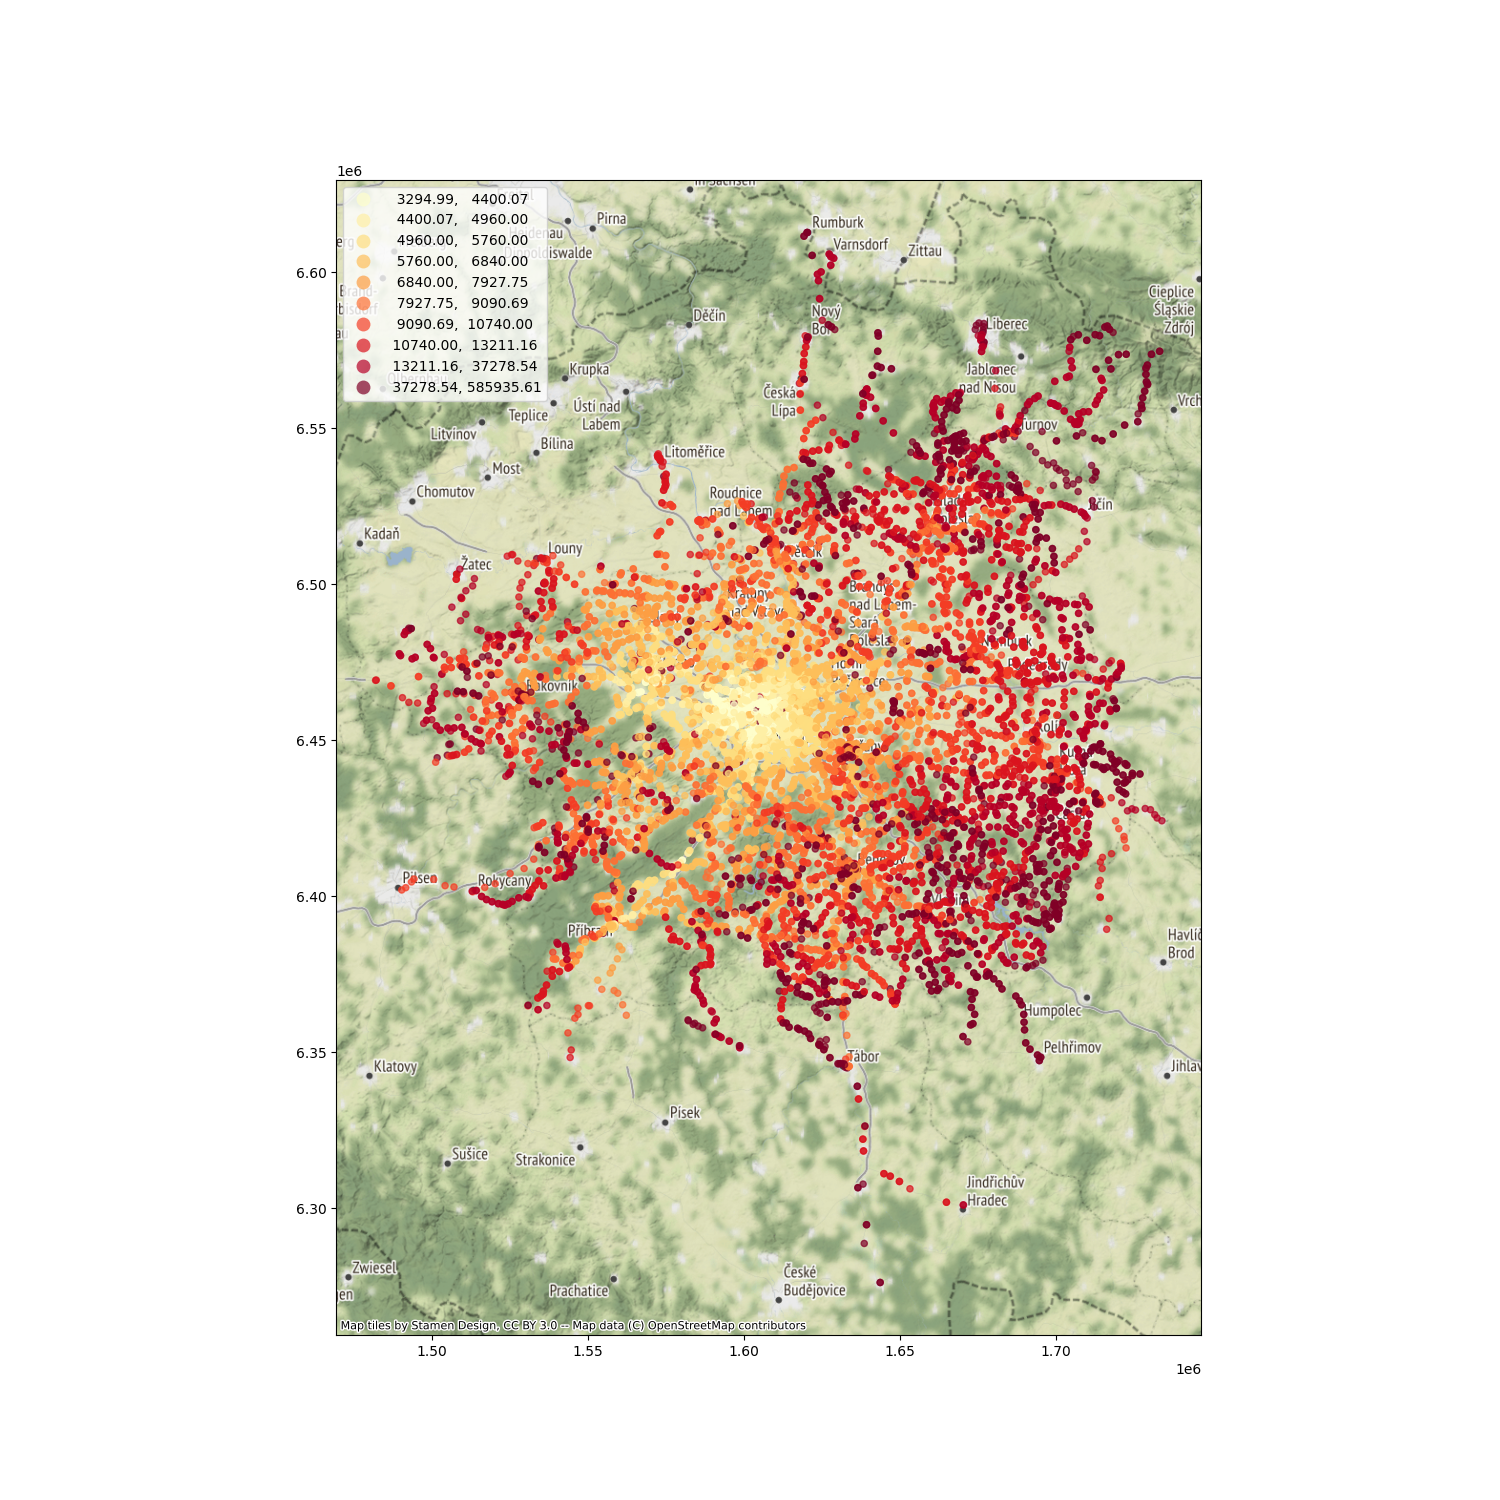
\includegraphics[width=\textwidth]{../img/staticStopsVisualization.png}
    \caption{Vizualizace dostupnosti na zastávkách z~Malostranského náměstí, Kladna a~Příbrami. Hodnoty v~legendě vyjadřují dostupnost v~sekundách.}
    \label{fig:gtfs-mostAccessibleStop}
\end{figure}

\subsubsection{Vizualizace míst}

Nejprve potřebujeme vybrat místa, která budeme vizualizovat. Místa budeme volit v~rastru. Tuto metodu jsme popsali i~s~optimalizací v~sekci~\ref{optim-body}.

Pro ohodnocení míst použijeme metodu popsanou v~sekci~\ref{zobecneni-ciloveZastavkyNaMista}.

Samotná vizualizace probíhá stejně jako vizualizace zastávek, viz obrázek~\ref{fig:gtfs-mostAccessiblePlace}.

\begin{figure}[ht]
    \centering
    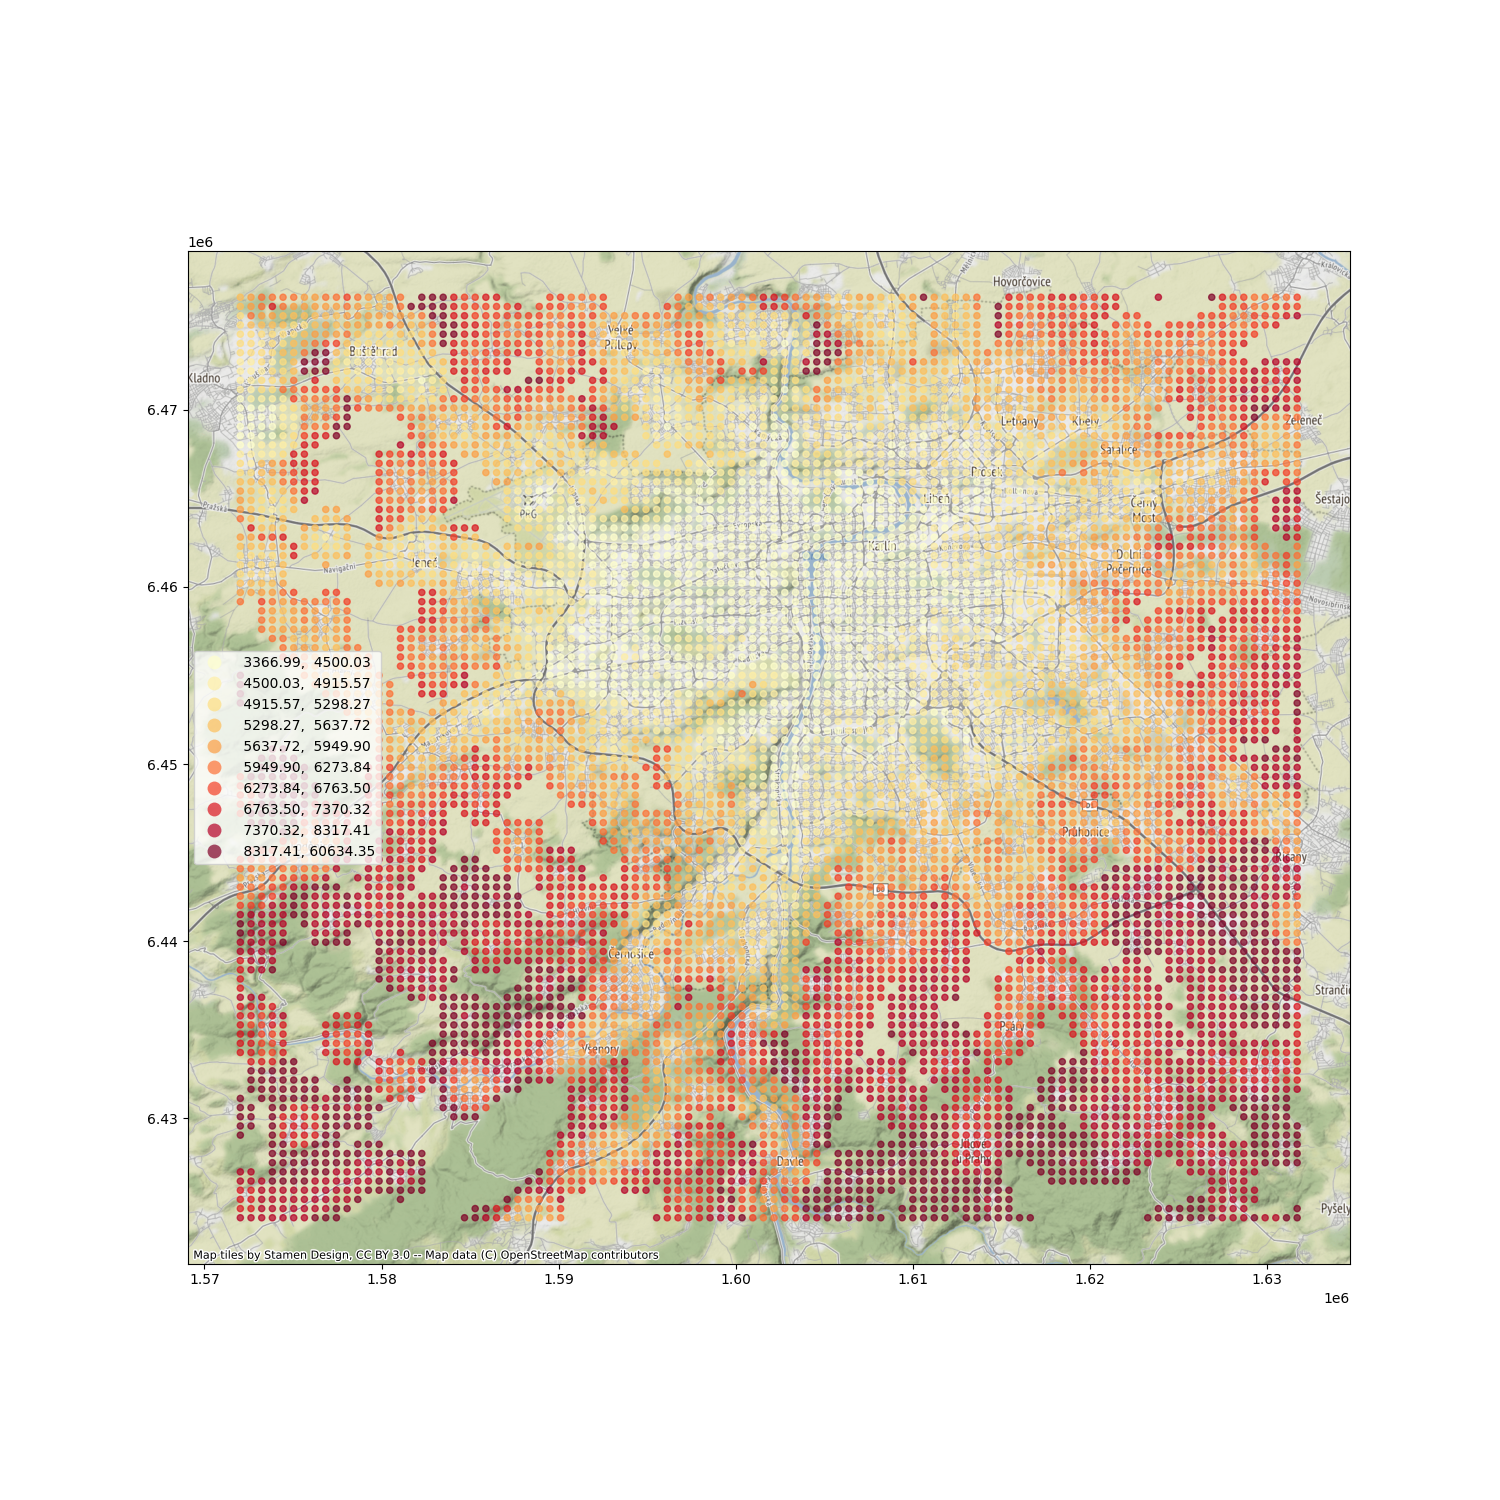
\includegraphics[width=\textwidth]{../img/staticPlaceVisualization.png}
    \caption{Vizualizace dostupnosti v~rastru 100~x~100 z~Malostranského náměstí, Kladna a~Příbrami. Hodnoty v~legendě vyjadřují dostupnost v~sekundách.}
    \label{fig:gtfs-mostAccessiblePlace}
\end{figure}


\section{Interaktivní vizualizace}\label{Interaktivni-vizualizace}

Dostupnost můžeme vizualizovat v~interaktivní mapě. Tím umožníme uživatelům nejen zobrazovat výsledky na mapě, ale také pohybovat se po mapě a~zjišťovat tak dostupnost na konkrétních místech.

Vizualizaci zpřístupníme uživatelům skrze webovou aplikaci. Z~toho důvodu jsme pro implementaci vizualizace zvolili jazyk JavaScript.

\subsubsection{Výběr knihovny}

Při implementaci této vizualizace budeme chtít využít existující knihovnu, abychom si ušetřili práci. Knihoven pro práci s~interaktivní mapou existuje mnoho. Zvážíme následující možnosti.

\begin{enumerate}
    \item Google map API. Google sice umožňuje využívat API po dobu prvního půl roku zdarma, obecně se ale jedná o~placenou službu.
    \item Mapquest. Placená knihovna, prvních 15 000 transakcí by mělo být zdarma.
    \item OpenLayers. Open-source knihovna, zcela zdarma.
\end{enumerate}

Preferovanou knihovnou je OpenLayers, neboť je jako jediná zdarma. Nenutí nás tedy vynucovat poplatky na uživatelích aplikace. Navíc nevynucuje žádné komerční závislosti pro případné další vývojáře naší aplikace.

\subsubsection{OpenLayers}

Knihovna OpenLayers používá jako výchozí projekci WGS84 (World Geodetic System). Stejná projekce je použita i~pro geografická data popsaná ve formátu GTFS. To nám ušetří práci s~případnými konverzemi projekcí.

Umožňuje kreslení na podklad map z~OSM (OpenStreetMap). Jedná se o~volně dostupné mapy, pro nás tedy ideální volba.

Pracuje s~vizualizačními vrstvami, není tedy problém přidat vrstvu obsahující vizualizované body a~vrstvu obsahující uživatelem zadaná vstupní místa pro výpočet dostupnosti.

Umí pracovat s~WebGL (Web Graphics Library), které umožňuje rychlejší vykreslování velkého množství bodů.

\subsubsection{Výsledná vizualizace}

Následující obrázky zobrazují interaktivní vizualizaci dostupností na zastávkách, viz obrázek~\ref{fig:ol-vizualizace-zastavek} a~vizualizaci dostupností na bodech v~rastru, viz obrázek~\ref{fig:ol-vizualizace-mist}.

\begin{figure}[ht]
    \centering
    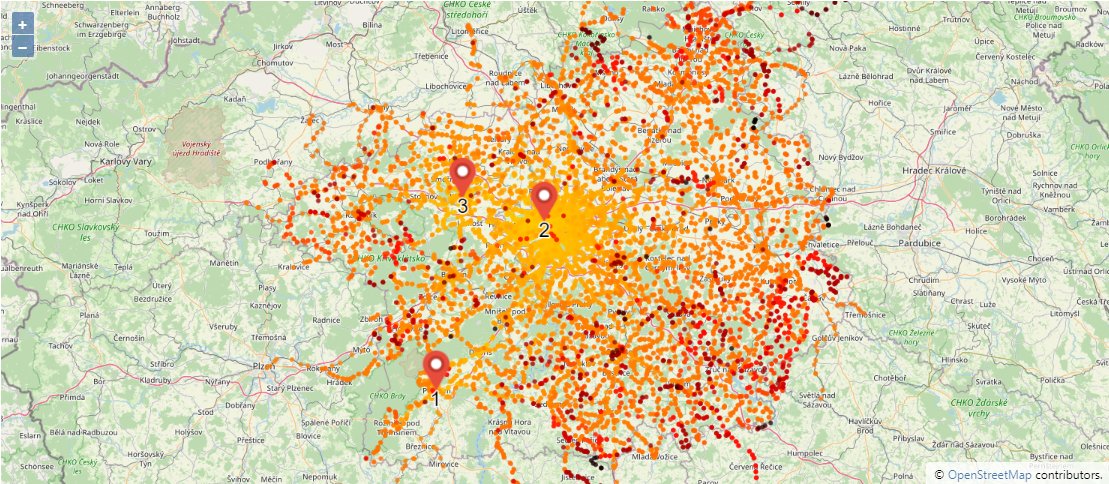
\includegraphics[width=\textwidth]{../img/interactiveStopVisualization.png}
    \caption{Interaktivní vizualizace dostupnosti na zastávkách z~Malostranského náměstí, Kladna a~Příbrami.}
    \label{fig:ol-vizualizace-zastavek}
\end{figure}

\begin{figure}[ht]
    \centering
    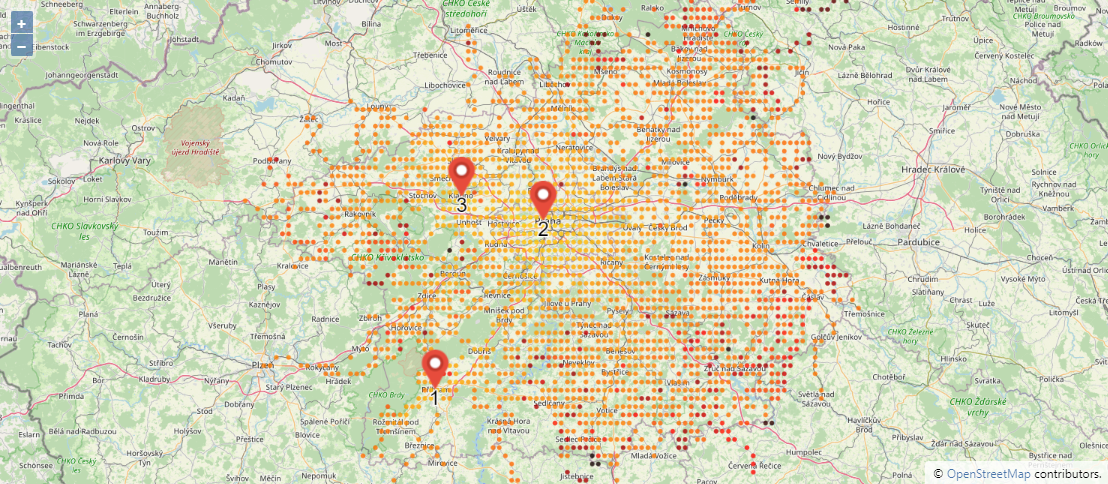
\includegraphics[width=\textwidth]{../img/interactivePlaceVisualization.png}
    \caption{Interaktivní vizualizace dostupnosti v~rastru 100~x~100 z~Malostranského náměstí, Kladna a~Příbrami.}
    \label{fig:ol-vizualizace-mist}
\end{figure}

\section{Možné vylepšení}

Spíše než vizualizace bodů by pro uživatele mohla být zajímavější možnost vizualizace pomocí jednolitého barevného filtru, který by překrýval mapu.

Základem takového filtru by byla dostupnost v~bodech. Dostupnost na místech mezi body bychom mohli interpolovat pomocí dostupností na okolních bodech.

\chapter{Implementace}\label{kapitola-Implementace}

Projekt jsme psali primárně s~použitím jazyku C\# pro verzi .NET Core 5. Součástí projektu je webová aplikace využívající framework ASP.NET, v~této části se objevují kromě jazyku C\# také jazyky Javascript, HTML a~CSS.

Náš projekt je koncipovaný jako knihovna a~webová aplikace. Knihovna zpracovává data jízdních řádů a~vypočítává dostupnost. Webová aplikace používá knihovní část a~umožňuje uživatelům zadávat vstupy, vizualizovat vypočtenou dostupnost a~procházet vizualizace v~interaktivní mapě.

Knihovní část aplikace je rozdělena na moduly, které vzájemně nezávisí na implementačních detailech a~tím je umožněna jejich snadná výměna. Tyto moduly nazýváme GTFSData, RaptorAlgo, StopAccessibility a~Config. Závislosti mezi moduly si můžeme prohlédnout na obrázku~\ref{fig:library-modules}.

\begin{figure}[ht]
    \centering
    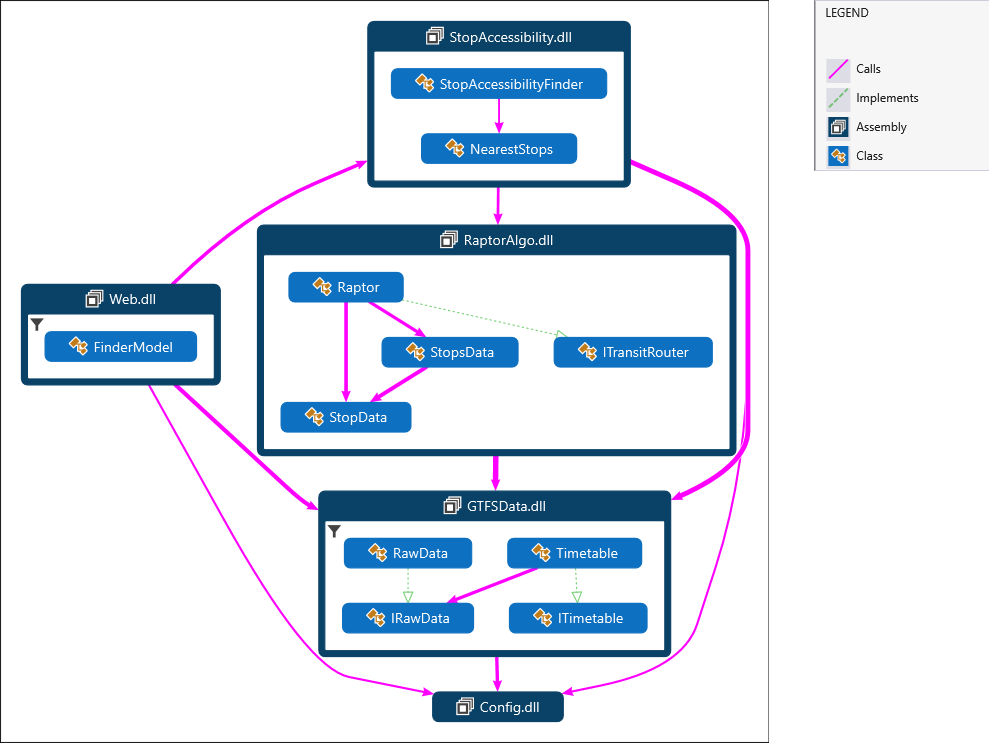
\includegraphics[width=\textwidth]{../img/codemap}
    \caption{Moduly aplikace a~jejich vzájemné propojení.}
    \label{fig:library-modules}
\end{figure}

Knihovní část projektu testujeme pomocí Unit Testů, psaných nástrojem XUnit. Testy pokrývají všechna základní použití knihovny, doplněné o~testy založené na chybách nalezených při vývoji.

% TODO: --------------v

% mozne rozsireni: o automaticky timezone
    % nepouziva Agency - alternativa v configu -- mozne rozsireni automatizaci


% update dat na webu---
\section{Modul GTFSData}

V~tomto modulu načítáme data jízdních řádů a~následně je zpracováváme. Součástí modulu jsou také pomocné funkce, které usnadňují práci s~projekcí WGS84 a~se zpracováním času.

Hlavní třídy modulu jsou:
\begin{itemize}
    \item RawData, která načítá data ze souborů formátu GTFS.
    \item Timetable, která načítá data do datových struktur vhodných pro vyhledávání.
\end{itemize}


\subsection{Třída RawData}\label{rawdata}

V~této třídě implementujeme myšlenky, popsané v~kapitole~\ref{kapitola-1}. Třída obsahuje specifikaci dat, která budeme načítat do paměti ze souborů formátu GTFS. Formát GTFS jsme popsali již v~sekci~\ref{gtfs-popis}.

Pro snazší parsování GTFS dat ve formě CSV používáme knihovnu \textbf{CsvHelper}. Tato knihovna, mimo jiné, určuje formát ve kterém popisujeme specifikaci parsovaných dat.

Při parsování \textbf{arrival\_time} a~\textbf{departure\_time} ze souboru \textbf{stop\_times} převádíme časy na \textbf{TimeSpan}, který nám umožňuje ukládat kromě času i~případné dny. Tímto způsobem ukládání dat se vyhneme problému s~časy, které přesahují klasický 24 hodinový formát.

Datum parsujeme do struktury \textbf{DateTimeOffset}. UTC posun určujeme v~pomocné třídě \textbf{TimeConverter}. Naše implementace určuje UTC posun dle hodnoty \textbf{UTCOffset} z~konfiguračního souboru.

\subsubsection{Možnost rozšíření o~jiný formát dat}

Implementaci třídy \textbf{RawData} můžeme nahradit, za podmínky dodržení specifikovaného rozhraní \textbf{IRawData}. To nám umožní pracovat s~daty jízdních řádu v~jiném formátu než je formát GTFS. Například bychom mohli pracovat s~daty ve formátu JDF, popsaném v~kapitole~\ref{kapitola-1}.


\subsection{Třída Timetable}\label{class-timetable}

Touto třídou reprezentujeme datové struktury uchovávající data jízdních řádů ve formě vhodné pro vyhledávání. Potřebná data jsme popsali již v~sekci~\ref{raptor-data}. Součástí této třídy jsou také metody, pomocí nichž stavíme zmíněné datové struktury.

Třída \textbf{Timetable} závisí na datech jízdních řádu, které ji poskytneme skrze rozhraní popsané výše v~sekci~\ref{rawdata}. Využívá návrhový vzor \textbf{Singleton}, který zajišťuje, že v~aplikaci bude existovat jen jediná instance této třídy. To je velice užitečné, neboť v~aplikaci pracujeme jen s~jedněmi daty jízdních řádů a~ty nechceme duplikovat.

\subsubsection{Popis datových struktur}

\begin{itemize}
    \item Struktura \textbf{Transfer}
    
    Touto strukturou popisujeme přestupy mezi zastávkami. Obsahuje čas přestupu a~zdrojovou a~cílovou zastávku.
    
    \item Struktura \textbf{Stop}

    Strukturou \textbf{Stop} reprezentujeme zastávky z~jízdních řádů. Obsahuje kolekci přestupů mezi zastávkami a~seznam tras, na kterých se zastávky nachází.
    
    Pro optimálnější hledání sousedních zastávek využíváme optimalizace popsané v~sekci~\ref{optim-sousedi}. Důsledkem této optimalizace je \textbf{Stop} potomkem \textbf{ISpatialData}.

    \item Struktura \textbf{StopTime}
    
    Tato struktura obsahuje informace o~příjezdu a~odjezdu z~odpovídající zastávky.

    \item Struktura \textbf{TripWithDate}\label{TripWithDate}
    
    Pomocí struktury \textbf{TripWithDate} reprezentujeme jízdu jedoucí v~konkrétním datu. Každá jízda obsahuje kolekci \textbf{StopTime}.
    
    Jelikož každá jízda může jet v~několika dnech, tedy i~několika datech, vedl by tento přístup k~redundantnímu ukládání kolekcí \textbf{StopTime}.
    
    Abychom tomu předešli, vytvořili jsme pomocnou strukturu \textbf{Trip}, která obsahuje informace sdílené mezi stejnými jízdami, včetně kolekce \textbf{StopTime}. Samotná struktura \textbf{TripWithDate} udržuje referenci na Trip a~přidává k~ní datum.
    
    \item Struktura \textbf{Route}
    
    Touto strukturou reprezentujeme trasu ve významu popsaném v~kapitole~\ref{kapitola-2}. Obsahuje množinu jízd, jedoucích po stejných zastávkách a~zastávky samotné.
    
    Jak jsme jíž zmínili v~sekci~\ref{raptor-data}, je nutné, abychom  obsažené jízdy udržovali uspořádané. K~tomu slouží metoda \textbf{SortTrips}.
\end{itemize}

\subsubsection{Fáze stavby datových struktur}

\begin{itemize}
    \item Inicializace
    
    Při inicializaci nastavujeme počáteční datum a~dobu platnosti dat z~jízdních řádů. Doba platnosti je vždy omezená a~dá se nastavit skrze konfigurační soubor.
    
    Po přidání zastávek dále inicializujeme \textbf{StopPositionLimits} a~stavíme \textbf{stopsInRTree}.
    
    Do vlastnosti \textbf{StopPositionLimits} ukládáme souřadnice obdélníku, který ohraničuje všechny zastávky. Toho využijeme později při vizualizaci.
    
    Strukturu \textbf{stopsInRTree} stavíme pro optimálnější vyhledávání, viz sekce~\ref{optim-sousedi}.
    
    \item Přidání zastávek --- metoda \textbf{AddStops}
    
    V~této fázi jen ukládáme zastávky z~dat jízdních řádů.
    
    \item Přidání tras --- metoda \textbf{AddRoutes}
    
    Během přidávání tras přidáváme také jízdy, které patří pod jednotlivé trasy.
    
    Jízdy vytváříme spojením dat z~různých souborů formátu GTFS pomocí klíčů. Konkrétně spojujeme \textbf{Calendar}, \textbf{CalendatDate} a~\textbf{Trips} přes klíč \textbf{service\_id} a~výsledek dále spojujeme se \textbf{StopTimes} přes klíč \textbf{trip\_id}. Vytvořené jízdy přidáváme do tras dle jednoznačného identifikátoru.
    
    Každá vytvořená jízda obsahuje \textbf{route\_id}. To samotné však k~jednoznačné identifikaci trasy nestačí, neboť definice GTFS trasy se liší od námi definované trasy. Jak jsme již zmiňovali v~kapitole~\ref{data-terminologie}, GTFS trasa může obsahovat jízdy, které jezdí přes různé zastávky.
    
    Abychom přiřadili jízdu pod správnou trasu, vygenerujeme si jednoznačný identifikátor trasy pomocí metody \textbf{GetRouteKey}, která jej generuje dle \textbf{route\_id} a~\textbf{id} každé ze zastávek na trase.
    
    Tato metoda pro každou trasu navíc vytváří \textbf{RouteStops}. Tedy seznam všech zastávek, přes které daná trasa vede.
    
    \item Přidání StopRoutes
    
    Metoda \textbf{AddStopRoutes} přidává pro každou zastávku seznam všech tras, které přes zastávku jezdí. Toto přidání nelze provést už při volání metody \textbf{AddStops}, neboť v~tu chvíli ještě nemáme uložené trasy.
    
    \item Odebrání nepoužitých zastávek
    
    Ukázalo se, že přinejmenším v~datech společnosti PID existují zastávky, přes které nevedou žádné trasy. Takové zastávky chceme odstranit, neboť zbytečně zpomalují výpočet. Samotné odstranění obstarává metoda \textbf{RemoveUnusedStops}.
    
    \item Generování přestupů\label{generovani-prestupu}
    
    Ke generování přestupů slouží metoda \textbf{GenerateTransfers}. Vzdálenost přestupů jsme omezili konstantou \textbf{MAX\_TRANSFER\_DISTANCE} a~rychlost přestupu určujeme konstantou \textbf{WALKING\_SPEED}. Obě konstanty jsou nastavitelné v~konfiguračním souboru.
    
    Pro hledání blízkých zastávek, mezi kterými definujeme přestupy, využíváme optimalizaci, popsanou v~sekci~\ref{optim-sousedi}. Bez využití optimalizace jsme nuceni porovnávat všechny dvojice zastávek a~to je velice neefektivní. Metoda \textbf{GenerateTransfers} je sice volaná maximálně jednou za běh programu, generování přestupů je však ze všech fází výpočetně nejnáročnější a~zvláště pro velké datasety je tato optimalizace nepostradatelná.
    
    Vzdálenost mezi zastávkami, pro zjednodušení, určujeme jako vzdálenost vzdušnou čarou. Možné zlepšení navrhujeme v~sekci~\ref{optim-prestupy}.
    
    Pro správné fungování vyhledávače je nutné, aby byly přestupy tranzitivní. Toho jsme docílili tak, že se na zastávky a~přestupy mezi nimi díváme jako na vrcholy a~hrany grafu. V~takovém grafu následně hledáme, pomocí DFS~(Depth-first search), komponenty silné souvislosti. Každá taková komponenta tvoří množinu zastávek, mezi kterými existují tranzitivní přestupy.
\end{itemize}

\subsubsection{Ukládání dat}

Stavba datových struktur, zejména generování přestupů, zabírá netriviální dobu při spouštění programu. Abychom nemuseli struktury opakovaně stavět při každém startu programu, bylo by vhodné si je někam uložit.

\begin{enumerate}
    \item Databáze

    Jednou z~možností datového úložiště je databáze. Při vyhledávání spojů však potřebujeme pracovat se všemi daty, dotazovat se vždy databáze by bylo příliš nepraktické. Navíc se dá předpokládat, že data jízdních řádů se vejdou do paměti.
    
    Databázi bychom mohli používat jen pro načtení dat při startu aplikace. Pak ale plně nevyužíváme výhody poskytované databází, mimo jiné proto, že data chceme pouze číst, ne do nich zapisovat. Samotná databáze nám tedy do aplikace zavádí zbytečnou složitost.
    
    \item Serializace
    
    Vhodnou alternativou k~databázi je serializace do souboru. Datové struktury postavíme jen jednou, při aktualizaci dat jízdních řádů a~serializujeme je. Následující spuštění aplikace deserializují datové struktury a~tím urychlí spouštění aplikace.
\end{enumerate}

V~naší aplikaci jsme pro ukládání dat použili serializaci do souboru. Data serializujeme do formátu JSON (JavaScript Object Notation). Jako serializační knihovnu jsme použili knihovnu \textbf{JSON.NET}, která oproti standardní serializaci poskytuje mnoho výhod. Dokáže například serializovat data s~cyklickými referencemi.

Samotná deserializace ze souboru však není příliš rychlá. Konkrétně, stavba \textbf{StopRoutes} je časově méně náročná, než jejich deserializace. Stavba \textbf{RouteStops} by mohla být také rychlejší než deserializace, museli bychom ji však nejprve oddělit od metody \textbf{AddStopRoutes}.

Při deserializaci velkých datasetů může docházet k~překročení maximální hloubky zanoření dat, serializovaných ve formátu JSON. Tu je však možné nastavit v~deserializačním konstruktoru.

\subsubsection{Práce s~kalendářem}

Naše prvotní implementace pracovala s~časem jako s~počtem sekund ve dni, stejně jako je to popsané v~článku \citep{raptor}. To se však ukázalo jako velice nepraktické. Nejen, že je reprezentace času jako čísla nevhodná. Tato reprezentace navíc neumožňovala rozlišení dnů ve kterých spoje jezdí, ani práci se spoji jedoucími přes půlnoc.

Rozhodli jsme se tedy čas reprezentovat ve strukturách k~tomu určených. Těmi jsou v~jazyku C\# \textbf{DateTimeOffset} a~\textbf{TimeSpan}. Tato reprezentace umožnila rozlišení jednotlivých dnů a~dokonce i~práci s~výjimkami v~jízdních řádech. Vyřešila také spoje jedoucí přes půlnoc, neboť k~takovému spoji lze jednoduše přičíst den.

% chybi popis class Calendar - neni prilis zajimave

Tento přístup však může mít i~nevýhody. Jako hlavní nevýhodu můžeme chápat složitější zadávání vstupu uživatelem v~případě, že uživatel pracuje přímo s~touto reprezentací, což se v~naší webové aplikaci děje.

Tato nevýhoda by se dala vyřešit abstrakcí uživatele od naší implementace. Problém ale je, jak by tato abstrakce měla vypadat. Pokud bychom nechali uživatele pracovat jen s~jednotlivými dny, není jasné, zdali tyto dny mají reprezentovat běžný den, či sváteční den. Navíc bychom, například pro prázdniny, museli pracovat se staršími daty, neboť jízdní řády v~takovém období bývají značně pozměněné.

Cenou za abstrakci by tedy byla práce s~nepřesnými či neaktuálními daty jízdních řádů. To však nechceme. Necháme tedy uživatele pracovat s~konkrétními daty. 


\subsection{Možné vylepšení}

\subsubsection{Lepší generování přestupů}\label{optim-prestupy}

V~této chvíli, během generování přestupů, měříme vzdálenost mezi zastávkami vzdušnou čarou. Tato vzdálenost, se však může velice odlišovat od vzdálenosti pěší chůzí. Příkladem mohou být například zastávky, které jsou sice poměrně blízko, jenže mezi nimi teče řeka. V~takovém případě se vzdálenost vzdušnou čarou může od pěší vzdálenosti lišit dramaticky.

V~ideálním případě bychom k~měření pěší vzdálenosti využili existující navigaci. Přímo pro mapy OSM bychom mohli použít některou z~navigací zmíněných na stránce \url{https://wiki.openstreetmap.org/wiki/Routing/offline\_routers}.

\subsubsection{Optimálnější uložení dat}

Datové struktury ukládající data ve třídě \textbf{timetable}, jsou psané v~objektově orientovaném stylu, neboť tento styl je dobře čitelný a~preferovaný v~prostředí jazyku C\#. Nevýhodou je však špatná datová lokalita, což vede k~více cache missům a~zpomaluje tak vyhledávání algoritmu RAPTOR.

Možným řešením je reprezentovat data v~datových strukturách přesně tak, jak jsou popsány v~článku \citet[Appendix A]{raptor}.
\section{Modul RaptorAlgo}

Tento modul implementuje algoritmus RAPTOR, viz kapitola~\ref{kapitola-2}, který používáme k~vyhledávání nejrychlejší cesty ze zadané zastávky, v~daný čas a~den, na ostatní zastávky. Implementace algoritmu nám navíc umožňuje zadávat více vstupních zastávek, čímž implementujeme zobecnění zastávky na místo, popsané v~sekci~\ref{raptor-zobecneni-vicePocatecnichZastavek}.


\subsection{Existující implementace}

Před samotnou implementací tohoto modulu jsme prozkoumali alternativní možnosti, které by nám mohli práci usnadnit. Tyto možnosti lze zařadit do dvou kategorií. Knihovny, umožňující vyhledávání v~jízdních řádech a~již existující implementace algoritmu RAPTOR.

\subsubsection{Knihovny}

Mezi námi zkoumané knihovny patří \textbf{OpenTripPlanner}\footnote{Dostupná na githubu, viz~\url{https://github.com/opentripplanner/OpenTripPlanner}} a~\textbf{Itinero}\footnote{Více informací lze dohledat na stránce \url{http://www.itinero.tech/}}.

\textbf{OpenTripPlanner} je knihovna psaná v~jazyku Java, což je jazyk, který spíše nepreferujeme pro tvorbu této aplikace.

\textbf{Itinero} je knihovna pro jazyk C\#.

Tyto knihovny však neřeší přímo náš problém. Abychom knihovny využili, museli bychom buď přepsat jejich část, nebo adaptovat naše řešení na možnosti knihoven.

Zmíněné knihovny řeší široké spektrum problémů a~jsou tedy velice komplexní. Z~toho důvodu jsou jakékoliv jejich úpravy značně složité. Nová implementace algoritmu RAPTOR se zdá být snazší, než přepisování části existující knihovny.

Adaptace našeho problému na možnosti knihoven se nezdá být vůbec snadná.

V~případě, že bychom přece jen byli schopni adaptaci zprovoznit, by toto řešení stále nebylo ideální. Naše poměrně malá knihovna by totiž závisela na mnohem větší knihovně, jejíž funkcionalitu bychom využívali jen ve velmi malé míře.

\subsubsection{Existující implementace algoritmu RAPTOR}\label{raptor-existujici-implementace}

Existující implementace by nám kromě ušetření času mohly poskytnout také optimalizované řešení, což by zaručilo rychlý běh algoritmu. Mezi nejrychlejší implementace algoritmu by patřily ty, napsané v~jazyku C/C++. Takové implementace bychom z~naší knihovny, psané v~jazyku C\#, mohli volat pomocí technologie \textbf{P/Invoke}.

\begin{enumerate}
    \item Implementace\footnote{Implementace je dostupná na githubu, viz \url{https://github.com/lviennot/hl-csa-raptor}} psaná v~jazyku C++. Tato implementace s~sebou bohužel nenese dokumentaci. Samotný kód se zdá být dosti nestrukturovaný, možná i~z~optimalizačních důvodů. To je však důvod, proč se provedení námi navrhovaných změn algoritmu zdá být v~této implementaci příliš pracné.
    \item Další dostupná implementace\footnote{Implementace je dostupná na githubu, viz \url{https://github.com/ducminh-phan/RAPTOR}}, psaná v~jazyku C++, bohužel také neobsahuje dokumentaci. Zdá se však, že je tato implementace trochu lépe strukturovaná. Při spuštění jsme však narazili na problém, že implementace předpokládá typované hodnoty v~GTFS datech. Formát GTFS však žádné typy nevynucuje. Například pro \textbf{trip\_id} knihovna předpokládá numerický typ, zatímco data společnosti PID jsou pod položkou \textbf{trip\_id} uloženy v~řetězcovém typu. Z~tohoto důvodu se nám ani nepodařilo spustit implementaci na našich datech.
    \item Poslední zkoumaná implementace\footnote{Implementace je dostupná na gitlabu, viz \url{https://gitlab.fel.cvut.cz/kasnezde/raptor}} je psaná v~jazyku Java. Tato implementace je dobře dokumentovaná a~její kód je přehledný. Tuto knihovnu jsme nevyužili, neboť naší aplikaci chceme psát v~jazyku C\#. Posloužila však jako inspirace pro naší implementaci a~usnadnila nám tak práci.
\end{enumerate}

Ze zmíněných implementací není žádná zcela vyhovující. Z~toho důvodu jsme se rozhodli implementovat si algoritmus RAPTOR sami.

\subsection{Třída Raptor}

Touto třídou reprezentujeme vyhledávač cest. Velká část implementace jen realizuje myšlenky popsané v~kapitole~\ref{kapitola-2}.

\subsubsection{Názvosloví pro práci s~časem}\label{NazvosloviCasu}

V~této třídě používáme často následující názvosloví pro práci s~různými časy.
\begin{itemize}
    \item \textbf{Walk time} --- doba trvání pěší cesty z~daného místa na zastávku.
    \item \textbf{Travel time} --- doba strávená na cestě jedoucím spojem.
    \item \textbf{Departure time} --- čas výjezdu spoje ze zastávky. 
    \item \textbf{Arrival time} --- čas příjezdu spoje na zastávku.
    \item \textbf{Start time} --- čas, od kterého začínáme vyhledávání.
    \item \textbf{Accessibility} --- dostupnost, neboli doba která uplynula mezi nejdřívějším \textbf{arrival time} a~\textbf{start time}, viz sekce~\ref{definice-dostupnosti}.
\end{itemize}

\subsubsection{Zajímavosti lišící se od implementace z~článku}

Vytvářením jízd pro každé datum kdy spoj jede, viz \textbf{TripWithDate} popsaný v~sekci~\ref{TripWithDate}, vzniká velký počet jízd. Tento nárůst počtu jízd může zpomalit běh metody \textbf{GetEarliestTripFromStop}, která vyhledává nejdřívější jízdu, na kterou můžeme z~dané zastávky nastoupit. Jednoduchou optimalizací je použití binárního vyhledávání pro nalezení hledané jízdy.

Metoda \textbf{Init} v~naší implementaci navíc označuje i~sousedy vstupní zastávky. Bez označení sousedů by algoritmus nenašel přestupy ze vstupní zastávky na zastávky v~jejím okolí. Důvodem je to, že v~první fázi algoritmu použijeme označenou vstupní zastávku k~označení tras a~zrušíme existující označení zastávek. Ve třetí fázi, kde aplikujeme přestupy z~označených zastávek, už není vstupní zastávka označena, tudíž přestupy z~ní nejsou nikdy využity.

Třída navíc obsahuje metodu \textbf{GetTravelTimeByStops}, která zpřístupňuje dostupnosti na zastávkách, které jsme vypočítali během vyhledávání. Tato metoda slouží jako propojení tohoto modulu s~modulem \textbf{StopAccessibility}, popsaným v~sekci~\ref{modul-StopAccessibility}.

\subsubsection{Možné zlepšení}

Tento modul nepředpokládá běžné využívání hodnoty \textbf{TotalRounds}, která omezuje počet přestupů v~nalezených cestách. Pro ohodnocení dostupnosti na všech dosažitelných místech sice tohoto omezení nevyužíváme, ale některé uživatele knihovny by vedle dostupnosti mohl zajímat i~počet přestupů. Tato změna by vyžadovala úpravu API tohoto modulu.


\subsection{Třída StopData}

Touto třídou reprezentujeme vypočtená data asociovaná se zastávkou. Jedná se zejména o~\textbf{multilabel arrivalTimes}, který pro každé kolo obsahuje nejdřívější příjezdové časy. Dále třída obsahuje \textbf{transfer}, \textbf{previousStop}, \textbf{trip}, která slouží k~vypisování cesty, viz sekce~\ref{RaptorAlgo-journey}.

\textbf{Multilabel arrivalTimes} rozšiřujeme líně, tedy až v~případě nutnosti. Příjezdové časy \textbf{multilabelu} pro neexistující a~nová kola vrací konstantu \textbf{UNREACHABLE}, která reprezentuje hodnotu nekonečno, jak jsme popsali již v~inicializaci algoritmu RAPTOR v~sekci~\ref{raptor-popisAlgo}.

Všechna vypočtená \textbf{StopData}, pro dosažitelné zastávky, uchováváme ve třídě \textbf{StopsData}, jenž slouží jako wrapper nad dictionary.


\subsection{Třída Journey} \label{RaptorAlgo-journey}

\textbf{Journey} jsme v~počáteční fázi vývoje používali k~vypisování cest mezi zadaným vstupním a~výstupním místem, kterou RAPTOR nalezl.

S~touto třídou je spojena logika tříd \textbf{Raptor} a~\textbf{StopData}. Když ve třídě \textbf{Raptor} dojde během vyhledávání k~aktualizaci \textbf{arrival\_time}, voláme na instanci \textbf{StopData}, asociované s~danou zastávkou, metodu \textbf{ArriveByTransfer} či \textbf{ArriveByTrip}. V~těchto metodách dochází k~uložení úseku cesty vedoucí na danou zastávku.

\subsubsection{Využití}

Tuto funkcionalitu v~naší aplikaci již nevyužíváme. Třídu \textbf{Journey} jsme však zachovali, neboť ji hojně využíváme při testování třídy \textbf{Raptor}.

Pokud by však uživatele naší knihovny zajímala cesta, kterou se dostanou ze zadaných míst na některé konkrétní místo. Můžeme cestu poměrně snadno vyhledat, využitím právě této třídy.

\subsection{Možné optimalizace}

Naše implementace algoritmu RAPTOR je napsaná v~jazyku C\#. Pro optimálnější běh algoritmu by však bylo vhodnější zvolit jazyk C++. Implementaci psanou v~jazyku C++ bychom mohli z~naší aplikace volat pomocí technologie P/Invoke, jak už jsme zmiňovali v~sekci~\ref{raptor-existujici-implementace}.

Algoritmus lze také optimalizovat využitím paralelizace, viz kapitola~\ref{raptor-paralelizace}.

\section{Modul StopAccessibility}\label{modul-StopAccessibility}

V~tomto modulu zobecňujeme vyhledávání implementované ve třídě \textbf{Raptor} podle metod popsaných v~kapitole~\ref{kapitola-3}. Konkrétně umožňujeme vyhledávání dostupnosti na libovolném výstupním místě, viz sekce~\ref{zobecneni-ciloveZastavkyNaMista}, vyhledávání z~více vstupních míst, viz sekce~\ref{zobecneni-viceVstupnichMist} a~výpočet dostupnosti v~intervalu, viz sekce~\ref{zobecneni-dostupnostVIntervalu}.

Uvnitř tohoto modulu stále pracujeme s~časovým názvoslovím, které jsme popsali již v~sekci~\ref{NazvosloviCasu}.


\subsection{Třída NearestStops}\label{class-NearestStops}

Třída \textbf{NearestStops} obsahuje pomocnou metodu \textbf{GetStopsWithWalkTime}. Touto metodou nalezneme sousední zastávky do maximální vzdálenosti, dané konstantou \textbf{DISTANCE\_LIMIT}, od zadaných souřadnic. Konstantu \textbf{DISTANCE\_LIMIT} načítáme z~konfiguračního souboru. Pro každou z~nalezených sousedních zastávek navíc počítáme čas který potřebujeme, abychom na zastávku došli pěší chůzí ze zadaných souřadnic. Pro efektivní vyhledávání sousedních zastávek využíváme optimalizaci zmíněnou v~sekci~\ref{optim-sousedi}.

\subsection{Třída StopAccessibilityFinder}

Základními interními metodami této třídy jsou metody \textbf{GetAvgTravelTimeByStop} a~\textbf{CalcAccessibility}.

\subsubsection{Metoda GetAvgTravelTimeByStop}

Za pomoci této metody agregujeme dostupnosti z~více zdrojů. V~případě, že jsou specifikovány váhy, agregujeme dostupnosti váženým průměrem. V~případě že váhy nejsou specifikovány, použijeme standardní průměr.

Uvnitř metody nejprve sčítáme dostupnosti na jednotlivých zastávkách a~odstraňujeme zastávky, které nejsou dostupné z~některého ze vstupních míst. Následně počítáme průměr z~dostupností.

\subsubsection{Metoda CalcAccessibility}\label{Metoda-CalcAccessibility}

V~metodě \textbf{CalcAccessibility} postupně procházíme vstupní zastávky. Pro každou vstupní zastávku nalezneme, s~pomocí metody \textbf{GetStopsWithWalkTime}, sousední zastávky, které dále využíváme k~výpočtu dostupností naší upravenou verzí algoritmu RAPTOR.

Každá vstupní zastávka může mít přidruženo větší množství počátečních dat s~časy. Dostupnosti pro každé datum a~čas počítáme zvlášť a~následně je průměrujeme metodou \textbf{GetAvgTravelTimeByStop}.

V~případě, že je metoda \textbf{CalcAccessibility} volaná s~parametry pro interval, počítáme navíc dostupnost pro každý čas v~intervalu. Tento postup jsme popsali již v~sekci~\ref{zobecneni-dostupnostVIntervalu}. Výsledky z~intervalu se opět průměrují metodou \textbf{GetAvgTravelTimeByStop}.

\subsubsection{Zobecnění vyhledávání na více vstupních míst}

Toto zobecnění jsme popsali v~sekci~\ref{zobecneni-viceVstupnichMist} a~zajišťují jej metody \textbf{GetAvgAccessByStop} a~\textbf{GetStatisticalAvgAccessByStop}. Obě metody využívají metodu \textbf{CalcAccessibility} pro ohodnocení jednotlivých zastávek a~výsledné dostupnosti průměrují metodou \textbf{GetAvgTravelTimeByStop}.

\subsubsection{Zobecnění vyhledávání na libovolné výstupní místo}

Toto zobecnění jsme popsali již v~sekci~\ref{zobecneni-ciloveZastavkyNaMista}. Zobecnění je implementováno metodami \textbf{GetAccessForCoords} a~\textbf{GetAccessForCoordNbors}.

Metoda \textbf{GetAccessForCoords} pro zadané souřadnice nejprve nalezne sousední zastávky a~čas potřebný pro jejich dosažení chůzí pomocí metody \textbf{GetStopsWithWalkTime} a~následně volá metodu \textbf{GetAccessForCoordNbors}.

Metoda \textbf{GetAccessForCoordNbors} je také součástí API, neboť pro vyhodnocení dostupnosti na velkém množství míst pro nás opakované hledání sousedních zastávek může znamenat výrazné zpomalení. Pro velké množství míst si můžeme sousední zastávky předpočítat a~následně využít tuto metodu. Využití této metody jsme popsali již v~sekci~\ref{optim-body}.

V~samotné metodě \textbf{GetAccessForCoordNbors} nejprve vypočteme dostupnosti pomocí metody \textbf{CalcAccessibility}. Následně procházíme všechny vstupní zastávky a~pro každou z~nich nalezneme zastávku sousedící se zadanými souřadnicemi, skrze kterou se na zadané souřadnice dostaneme nejrychleji. Dostupnost takto nalezené zastávky nám vyjadřuje dostupnost ze vstupní zastávky na zadané souřadnice. Ohodnocením místa na zadaných souřadnicích je vážený průměr dostupností ze všech vstupních zastávek.

\subsection{Možná zlepšení}

\subsubsection{Lepší výpočet vzdálenosti}

Aktuálně počítáme vzdálenost jako vzdálenost vzdušnou čarou. To je dosti nepřesné. Na stejný problém jsme narazili při generování přestupů a~navrhované řešení jsme popsali v~sekci~\ref{optim-prestupy}.

\subsubsection{Redundance u~přidružení více dat s~časy ke vstupní zastávce}

Každá vstupní zastávka může mít přidružených více počátečních dat s~časy. V~tuto chvíli počítáme dostupnost pro každý z~časů zvlášť. To však může být velice neefektivní.

V~případě, že by uživatel zadal stejné časy pro po sobě jdoucí všední dny, například pondělí a~úterý, může se stát že se pro tyto dny jízdní řády vůbec neliší. Počítáme tedy dvakrát to samé.

Takových případů může být více. Prozatím nenavrhujeme žádné řešení, jen poukazujeme na možnou redundanci.

% upravoval jsem API, puvodni navrh nebyl vhodny pro pouziti z webu - asi nema cenu zminovat
\section{Modul Web}

V~tomto modulu implementujeme webovou aplikaci, která zpřístupňuje naši knihovnu, pro výpočet dostupnosti, běžným uživatelům. Součástí tohoto modulu je také implementace interaktivní vizualizace, popsané dříve v~sekci~\ref{Interaktivni-vizualizace}.

\subsection{Části webové aplikace}

Před samotným popisem modulu si popíšeme části webové aplikace, které budeme implementovat.

Hlavní stránkou webové aplikace je stránka \textbf{Finder}, skrze níž mohou uživatelé vyhledávat dostupnost, viz obrázek~\ref{fig:Finder}.

\begin{figure}[ht]
    \centering
    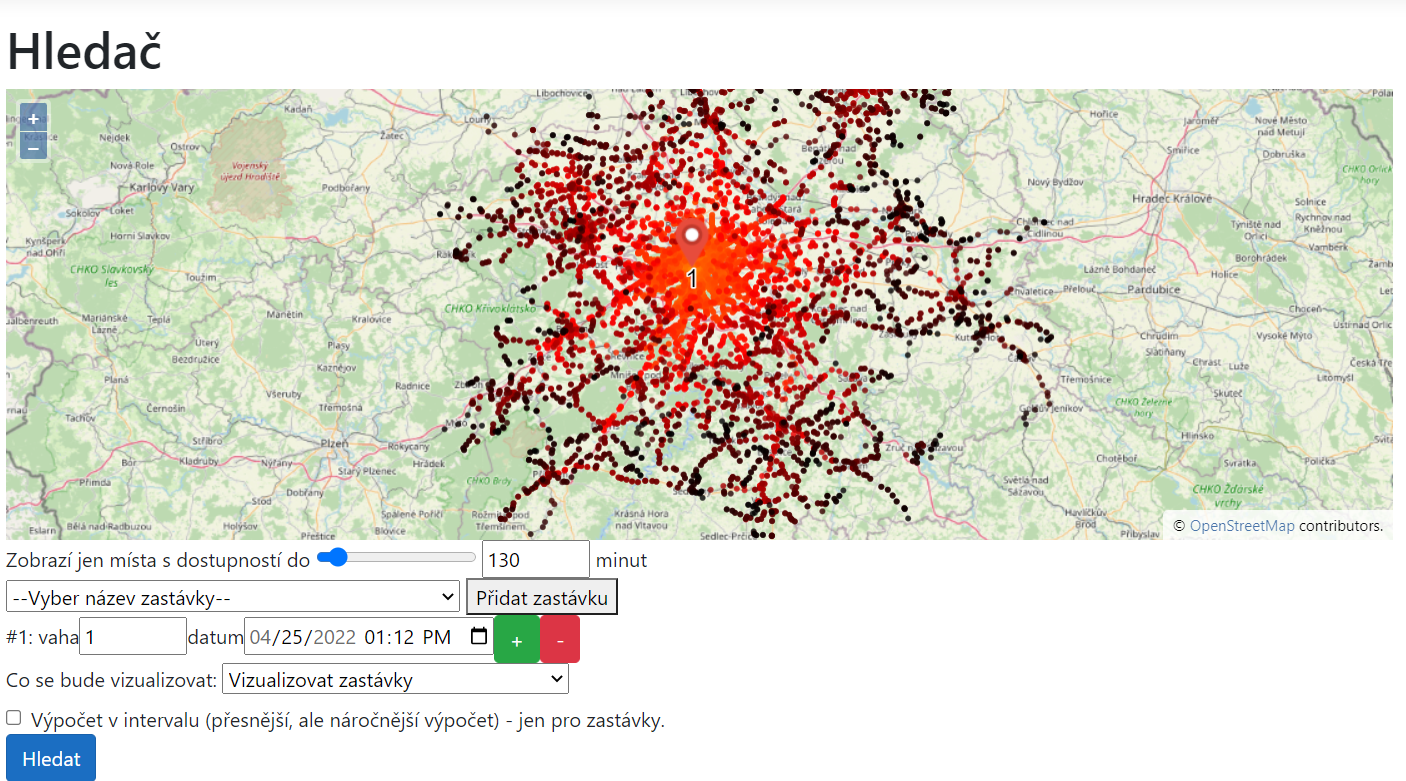
\includegraphics[width=\textwidth]{../img/finder.png}
    \caption{Stránka Finder.}
    \label{fig:Finder}
\end{figure}

\subsubsection{Značky}
% mozna pridat obrazek ikony markeru se zdrojem

Přidání značky reprezentující vstupní místo je možné dvěma způsoby. Kliknutím do mapy, nebo výběrem zastávky ze seznamu všech zastávek.

Vybrané vstupní místo lze odstranit kliknutím na značku asociovanou k~tomuto místu.

Značky lze po mapě přesouvat myší.

\subsubsection{Formulář se vstupními místy}

Formulář se vstupními místy generujeme dynamicky. Pro každé nové vstupní místo přidáváme položku.

S~každým vstupním místem asociujeme váhu a~skupinu dat s~časy. Váhu používáme k~výpočtu váženého průměru. Data s~časy určují dobu, kdy ze zastávky chceme vyjíždět. Data s~časy lze přidávat tlačítkem $+$ a~odebírat tlačítkem $-$.

Vizualizovat můžeme zastávky, body nebo obojí.

Při vizualizaci zastávek vizualizujeme všechny zastávky, které dostupné ze vstupních míst.

Při vizualizaci bodů vytváříme čtvercový rastr o~rozlišení daném konstantou \textbf{VisualisedRasterPointsResolution}, viz sekce~\ref{optim-body}. Mezi vizualizovanými body jsou jen ty, které jsou v~maximální vzdálenosti, dané konstantou \textbf{NearestStopsDistanceInMeters}, od nejbližší dostupné zastávky. Konstanty pochází z~konfiguračního souboru.

Uživatel si může zažádat o~výpočet v~intervalu, viz metoda \textbf{CalcAccessibility} v~sekci~\ref{Metoda-CalcAccessibility}. Takový výpočet je náročnější než klasický výpočet, jeho výsledky jsou však přesnější.

Formulář lze odeslat ke zpracování kliknutím na tlačítko \textbf{Hledat}. Po vypočtení dostupnosti dojde k~vizualizaci bodů na mapě.

Pokud byla některá značka na místě vzdáleném o~více než \textbf{NearestStops\hyp{}DistanceInMeters} od nejbližší zastávky, dojde k~vypsání chyby a~označení vstupního místa způsobujícího chybu, viz obrázek~\ref{fig:Finder-chyba}.

\begin{figure}[ht]
    \centering
    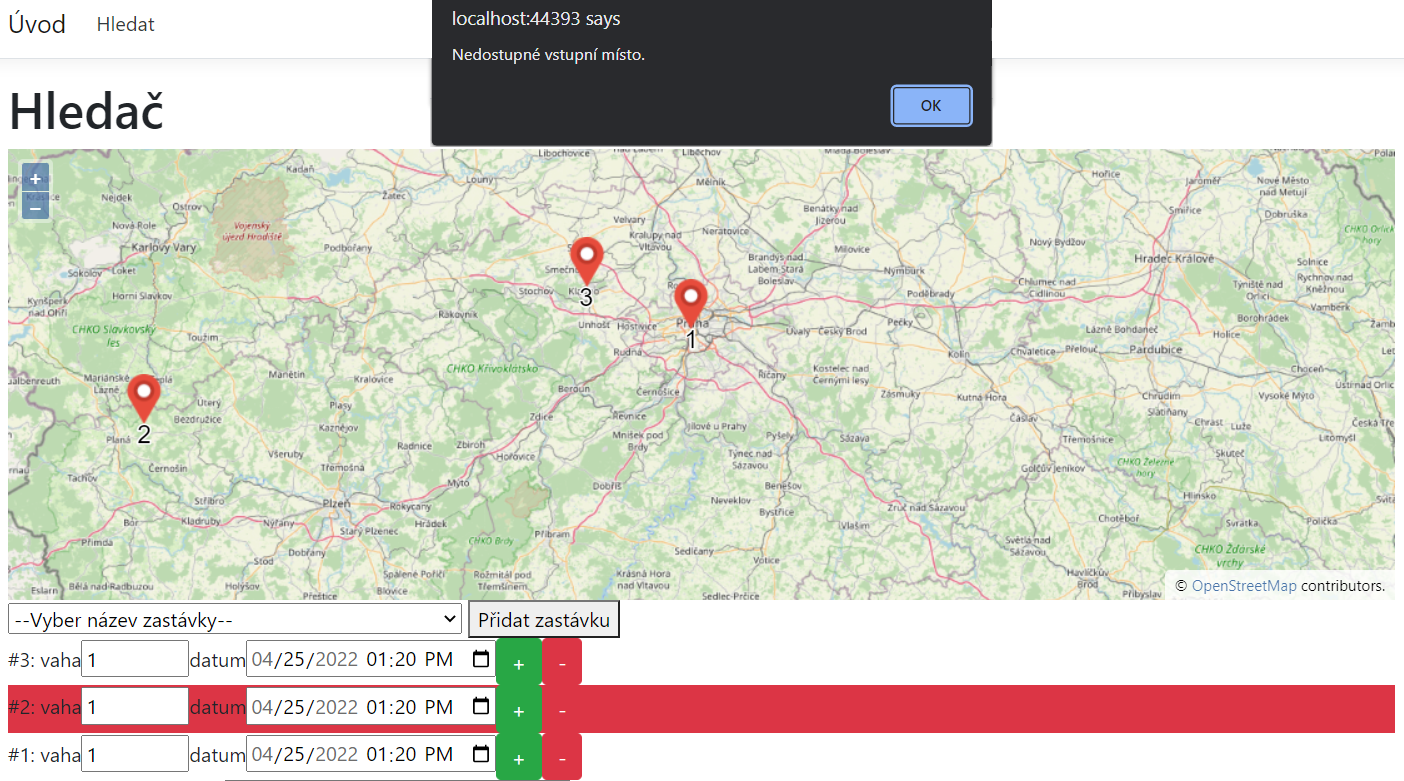
\includegraphics[width=\textwidth]{../img/finder-chyba.png}
    \caption{Hlášení chyby při zadání nedostupného místa.}
    \label{fig:Finder-chyba}
\end{figure}

\subsubsection{Výsledná dostupnost}

Dostupnost na vizualizovaných místech barevně rozlišujeme. Tmavě jsou označena méně dostupná místa a~světle jsou označena dostupnější místa.

Pro snazší hledání dostupných míst jsme zavedli posuvník, kterým lze omezit maximální vizualizovanou dostupnost. Barvy na vizualizovaných místech překreslujeme v~závislosti na aktuálně nastavené maximální dostupnosti.

Nejdostupnější místa vypisujeme v~tabulce pod formulářem.


\subsection{Backend}

Náš backend je postavený nad webovým frameworkem ASP.NET Core. Framework ASP.NET jsme zvolili, neboť naše knihovní část je napsaná v~jazyku C\# a~ASP.NET je velice populárním frameworkem pro tento programovací jazyk.

\subsubsection{Volba modelu}

Framework ASP.NET umožňuje vytvářet webové aplikace ve dvou modelech, \textbf{ASP.NET MVC} a~\textbf{Razor Pages}.

\begin{itemize}
    \item \textbf{ASP.NET MVC} je postavený na návrhovém vzoru Model–view–controller, který odděluje UI, data a~logiku. Použití tohoto návrhového vzoru sice zvyšuje flexibilitu, cenou je však vyšší složitost. Důsledkem těchto vlastností je tento model vhodný spíše pro větší aplikace.
    \item Model \textbf{Razor Pages} je jednodušší, odděluje pouze UI a~logiku.
\end{itemize}

My jsme zvolili model \textbf{Razor Pages}, neboť naše aplikace není příliš rozsáhlá a~MVC by nám do aplikace zanášelo zbytečnou složitost.

\subsubsection{Zpřístupnění knihovny jako Dependency Injection služby}

Abychom mohli využívat námi implementovanou knihovnu pro výpočet dostupnosti, musíme ji nejprve zpřístupnit pro webovou aplikaci.

Toho docílíme načtením potřebných modulů jako služby. Načítání služby obstarává metoda \textbf{ConfigureServices} uvnitř třídy \textbf{Startup}. Každá služba má přiřazenou životnost, my používáme typy životnosti \textbf{singleton} a~\textbf{scoped}.

\begin{itemize}
    \item \textbf{Singleton} --- existuje jedna instance pro všechny webové dotazy.
    \item \textbf{Scoped} --- existuje nová instance pro každý webový dotaz.
\end{itemize}

Načtené služby jsou nám následně zpřístupněny za pomoci \textbf{Dependency Injection} skrze konstruktor.

\subsubsection{Stránka Finder}

\textbf{Finder} je hlavní stránka naší webové aplikace.

Metodu \textbf{OnPost} využíváme ke zpracování vstupu, zadaného uživatelem do formuláře.

Jelikož počet vstupních zastávek zadaných uživatelem není předem známý, potřebujeme data získávat z~dynamicky rozšiřitelného formuláře. To bohužel znemožňuje použití \textbf{bindování}, které ASP.NET poskytuje pro uložení uživatelského vstupu přímo do atributů. Místo toho použijeme pro přenos dat formát \textbf{JSON} (JavaScript object notation).

Pro vizualizaci bodů potřebujeme znát sousedy těchto bodů. Tyto sousedy si můžeme vyhledat jednou a~pracovat s~nimi v~dalších výpočtech, viz sekce~\ref{optim-body}. Toto je implementováno ve třídě \textbf{PointsWithNeighbors}.

\subsubsection{Třída DataUpdater}\label{trida-DataUpdater}

Třída \textbf{DataUpdater} zajišťuje aktualizaci dat jízdních řádů.

Metoda \textbf{GetTimetable} poskytuje přístup k~instaci třídy \textbf{Timetable}, popsané v~sekci~\ref{class-timetable}.

K~aktualizaci dat dojde v~případě, že je nastavený \textbf{ShouldUpdate} v~konfiguračním souboru nebo pokud chybí serializace dat jízdních řádů.

Během aktualizace stahujeme zazipovaná data z~adresy dané konstantou \textbf{GTFSSourceURI} a~následně je extrahujeme do složky na cestě dané konstantou \textbf{PathToGTFSFolder}. Konstanty pochází z~konfiguračního souboru.

\subsubsection{Možné zlepšení}

Pokud bychom chtěli kromě webové aplikace vytvářet také mobilní či desktopovou aplikaci, mohli bychom využít ASP.NET Web API, které umožňuje vytváření \textbf{REST API}. Tento přístup jsme nevyužili, neboť bychom vedle samotného Web API museli vytvářet ještě samotnou webovou aplikaci a~to by do naší aplikace zanášelo další složitost.


\subsection{Frontend}

Jako programovací jazyk pro frontend jsme zvolili populární \textbf{JavaScript}. Interaktivní mapu vytváříme s~pomocí knihovny \textbf{OpenLayers}. Ke stylování HTML prvků používáme knihovnu \textbf{Bootstrap 4}.

Všechen JavaScriptový kód pro stránku \textbf{Finder} se nachází v~souboru \textbf{map.js}. Vedle pomocných funkcí a~konstant jsou v~souboru obsaženy dvě hlavní třídy, \textbf{Form} a~\textbf{OLMap}.


\subsubsection{Třída Form}

Tato třída obsahuje metody pro práci s~formulářem, do kterého uživatel zadává vstupní místa.

Formulář je dynamický, díky čemuž můžeme za běhu přidávat vstupní místa, případně data s~časy asociované se vstupními místy. To zajišťují metody \textbf{addField} a~\textbf{removeField}.

Data z~formuláře odesíláme na server ve formátu \textbf{JSON}. Zpracování dat a~jejich \textbf{serializaci} obstarává metoda \textbf{submit}. Odpověd ze serveru je také zpracovaná touto metodou. V~případě, že uživatel zadal nedosažitelné vstupní místo, volá se metoda \textbf{unreachableTargetHandler}. Pokud vše proběhlo v~pořádku, vrátí se nám ze serveru dostupnost pro všechny zastávky či místa, s~tou dále pracujeme v~metodě \textbf{handleResponse}.

Framework ASP.NET obsahuje ochranu proti CSRF (Cross-Site Request Forgery) útokům pomocí tokenu \textbf{\_\_RequestVerificationToken} vloženého do fomuláře jako hidden field. Abychom umožnili posílání dat z~JavaScriptu na server, musíme s~nimi posílat také tento token.


\subsubsection{Třída OLMap}

V~této třídě vytváříme interaktivní mapu pomocí knihovny \textbf{OpenLayers}.

V~konstruktoru skládáme mapu z~vrstev. \textbf{TileLayer} obsahuje mapy z~OSM. \textbf{MarkerLayer} slouží pro zobrazení značek, které uživatel umísťuje do mapy. \textbf{VisualizationLayer} slouží k~zobrazeni bodů s~barvou v~závislosti na jejich dostupnosti.

V~konstruktoru dále nastavujeme funkcionalitu potřebnou pro přesouvání značek umístěných v~mapě. Logiku pro přesouvání značek zajišťují metody \textbf{updateFormOnMarkerMovement} a~\textbf{changeCursorOnMarkerMovement}.  

Třída dále obsahuje metodu \textbf{addOrRemoveMarker}, která reaguje na kliknutí do mapy a~umožňuje tak přidávání a~odebírání značek.

\subsubsection{Možné vylepšení}

Přestože naše knihovna dokáže vypočítat dostupnost pro zcela libovolné místo, naše webová aplikace to uživatelům neumožňuje. Webová aplikace umožňuje jen vyhodnocení dostupnosti v~předem daných bodech a~na zastávkách.

Pro uživatele by mohlo být zajímavé řešení, které by zobrazovalo dostupnost pro místo na které ukazuje kurzor myši.

Pokud bychom posílali dotaz pro výpočet dostupnosti při každém pohybu myši, nejspíše by došlo snadno k~zahlcení serveru. Ideální by bylo provádět tento výpočet u~klienta. Problém je však v~tom, že kód počítající dostupnost je psaný v~C\# na straně serveru.

Možné řešení je přepsat kód do JavaScriptu, tím ale kód duplikujeme a~tomu se chceme spíše vyhnout.

Lepším řešením by bylo využít framework \textbf{Blazor}, který umožňuje spouštění C\# kódu v~klientském prohlížeči skrze technologii \textbf{WebAssembly}.

%knihovnu OpenLayers mam stazenou celou, stahuji ji i uzivatele, da se vsak zaridit, aby se stahovaly jen vyuzivane moduly - `in production: create own lib of used modules

\section{Modul Config}
% vsude chybi ref na config??----------

Tento modul zpřístupňuje data potřebná ke konfiguraci naší aplikace.
% mozna dopsat neco jako -> dynamicke zmeny: napr. obsah konstant - upravuji vyhledavani | ukladani souboru | ...


\subsubsection{Konfigurační soubor}

Konfigurační soubor \textbf{appsettings.json} obsahuje konfigurační data, která lze ručně modifikovat.

Soubor je psaný ve formátu JSON. Formát JSON jsme zvolili, neboť je poměrně populární, dobře čitelný a~stručný, srovnáme-li ho například s~formátem XML (Extensible Markup Language).


\subsubsection{Načtení dat konfiguračního souboru}

Načítání dat zajišťuje třída \textbf{AppConfig}. V~této třídě jsme pomocí statického konstruktoru zajistili, že k~načtení konfiguračních dat dojde při prvním přístupu k~jejich hodnotám.

Třída \textbf{AppPath} nám zajišťuje, že můžeme se souborovými cestami pracovat relativně vůči adresáři projektu.

V~původním návrhu jsme soubor \textbf{appsettings.json} nechávali kopírovat do výstupního adresáře a~následně jsme pracovali s~kopii tohoto souboru. To však vedlo ke vzniku kopie pro každý modul a~dokonce docházelo k~chybám, kdy nedošlo k~překopírování souboru \textbf{appsettings.json} do některého z~modulů. Rozhodli jsme se tedy pracovat s~tímto souborem přímo.


\subsubsection{Přístup k~načteným datům}

Pro přístup k~datům jsme vytvořili datovou třídu \textbf{AppSettings}. Položky této třídy zrcadlí strukturu souboru \textbf{appsettings.json}. Abychom zajistili typovaný přístup k~datům, využíváme \textbf{options pattern}\footnote{Detailní popis lze najít na adrese \url{https://docs.microsoft.com/en-us/dotnet/core/extensions/options}}.

Práci nám usnadňuje rozšíření \textbf{Microsoft.Extensions.Configuration}.

Instanci \textbf{AppSettings} vytváříme ve třídě \textbf{AppConfig}, ta ji také zpřístupňuje skrze položku \textbf{appSettings}.

\chapter{Výsledky}

V~předchozích kapitolách jsme již ukázali, jak vypadají vizualizace dostupnosti. Pracovali jsme však jen s~jízdními řády společnosti PID. Jak jsme však zmiňovali v~úvodu, naše aplikace má za cíl pracovat s~jízdními řády z~různých lokalit.

V~této kapitole si ukážeme, jak funguje naše aplikace pro data z~různých lokalit. Dále zmíníme, jak dlouho trvají výpočty s~jedním vstupním místem na procesoru \textbf{i5-6300U}. Pro intervalové výpočty volíme třiceti minutové okolí vstupního času s~intervalem o~délce jedné minuty.


\section{Chicago}

GTFS data pro město Chicago jsou dostupná na stránce transitfeed\footnote{Konkrétně na \url{https://transitfeeds.com/p/chicago-transit-authority/165}}.

Data jsou svou velikostí srovnatelná s~daty poskytovanými společnosti PID. Data společnosti PID obsahují zhruba 16~000~zastávek a~83~000~jízd. Data města Chicago obsahují 11~000~zastávek a~94~000~jízd.

Průměrně trvá:
\begin{itemize}
    \item Vyhodnocení dostupnosti na zastávkách: 210~ms.
    
    \item Vyhodnocení dostupnosti v~intervalu na zastávkách: 2~560~ms.
    
    \item Výpočet sousedů bodů v~rozlišení 100~x~100: 6~550~ms.
    
    \item Vyhodnocení dostupnosti pro body v~rozlišení 100~x~100: 215~ms
\end{itemize}

%odkaz na obrazky?

\begin{figure}[ht]
    \centering
    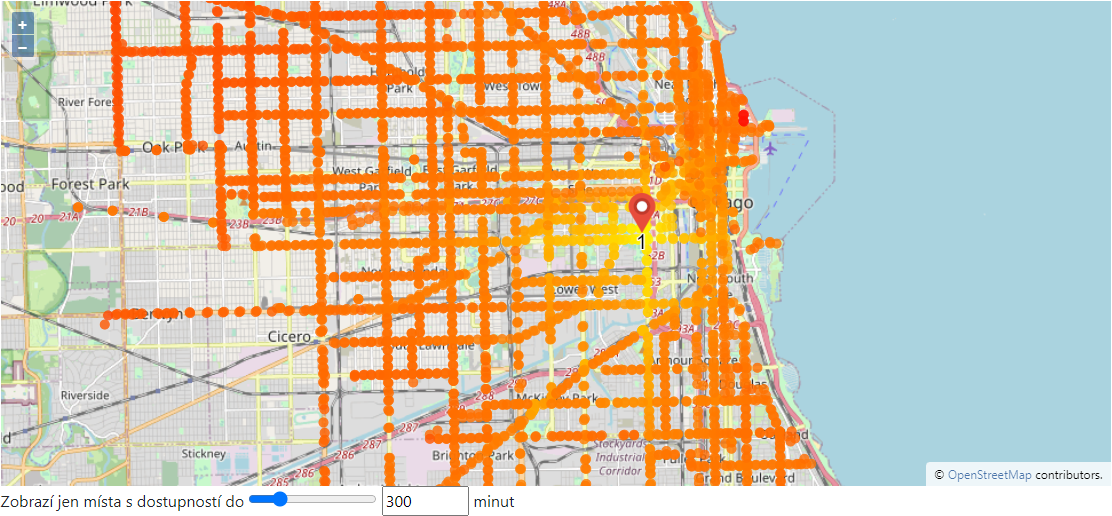
\includegraphics[width=\textwidth]{../img/Chicago-zastavky.png}
    \caption{Vizualizace dostupnosti do 300 minut na zastávkách v~Chicagu.}
    \label{fig:Chicago-zastavky}
\end{figure}

\begin{figure}[ht]
    \centering
    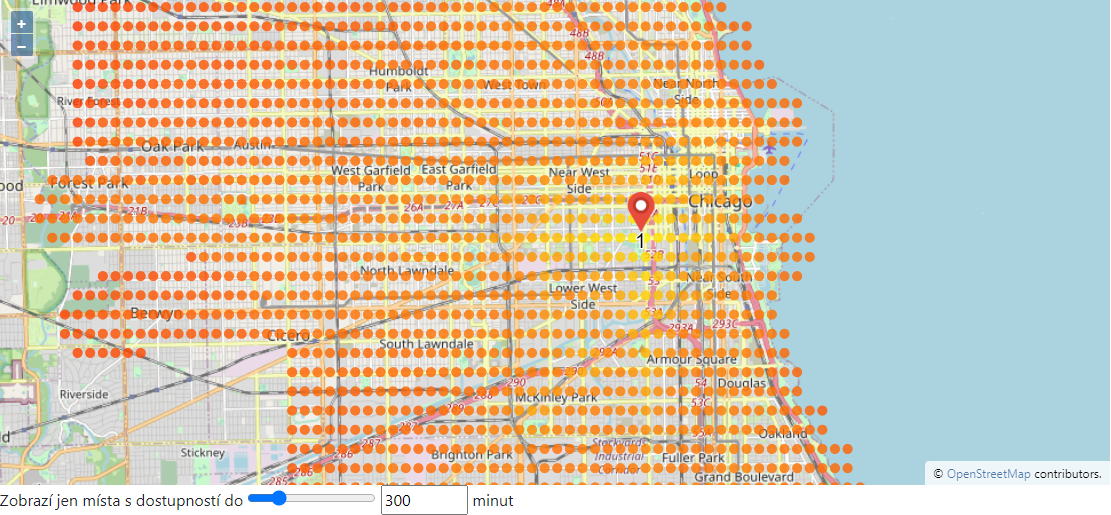
\includegraphics[width=\textwidth]{../img/Chicago-body.png}
    \caption{Vizualizace dostupnosti do 300 minut na bodech v~rastru pro Chicago.}
    \label{fig:Chicago-body}
\end{figure}


\section{Německo}

GTFS data pro celé Německo jsou dostupná na stránce \url{https://gtfs.de/en/feeds/de\_nv/}.

Jedná se o~největší jednotný dataset, který se nám podařilo nalézt. Ve srovnání s~daty společnosti PID obsahují tato data zhruba 27x~více zastávek a~16x~více jízd.

Průměrně trvá:
\begin{itemize}
    \item Vyhodnocení dostupnosti na zastávkách: 17.5~s.
    
    \item Vyhodnocení dostupnosti v~intervalu na zastávkách: 100~s.
\end{itemize}

\subsection{Problémy s~velkými daty}

Použití takto objemných dat však není jednoduché.

Zpracování a~serializace dat nám, za použití optimalizace popsané v~sekci~\ref{optim-prestupy}, trvala zhruba 2 hodiny.

Při deserializaci jsme museli navýšit maximální hloubku zanoření při čtení formátu JSON a~s~tím i~související velikost zásobníku.

Přetečení zásobníku jsme museli řešit i~na frontendu, konkrétně v~JavaScriptové funkci \textbf{Math.min}. 

Nakonec se nám podařilo vizualizovat zastávky, viz~\ref{fig:Nemecko-vse} a~\ref{fig:Nemecko-Berlin}. Pro takto velká data však naše aplikace není stavěná.

Vyhledávání je příliš pomalé pro praktické využití.

Nejsme schopni rozumně vizualizovat body v~rastru, neboť území Německa je poměrně velké a~body v~rozlišení 100~x~100 jsou vzájemně příliš vzdáleny. Větší rozlišení by vyžadovalo déle trvající předvýpočet sousedů či optimalizaci hledání sousedů.

\begin{figure}[ht]
    \centering
    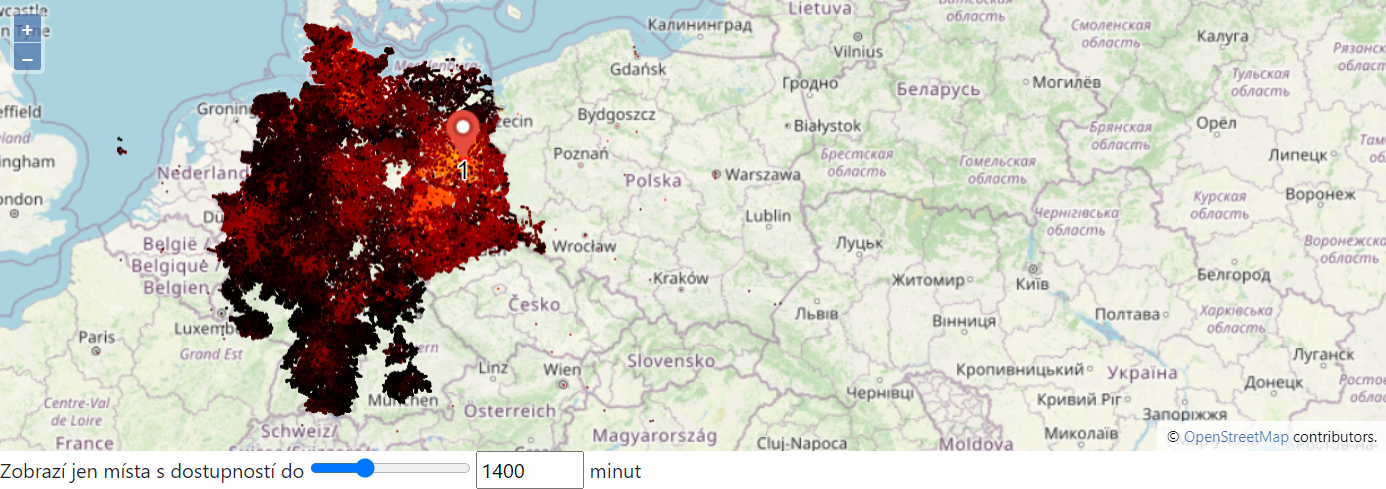
\includegraphics[width=\textwidth]{../img/Nemecko-Vse.png}
    \caption{Vizualizace dostupnosti do 1400 minut na zastávkách v~Německu.}
    \label{fig:Nemecko-vse}
\end{figure}

\begin{figure}[ht]
    \centering
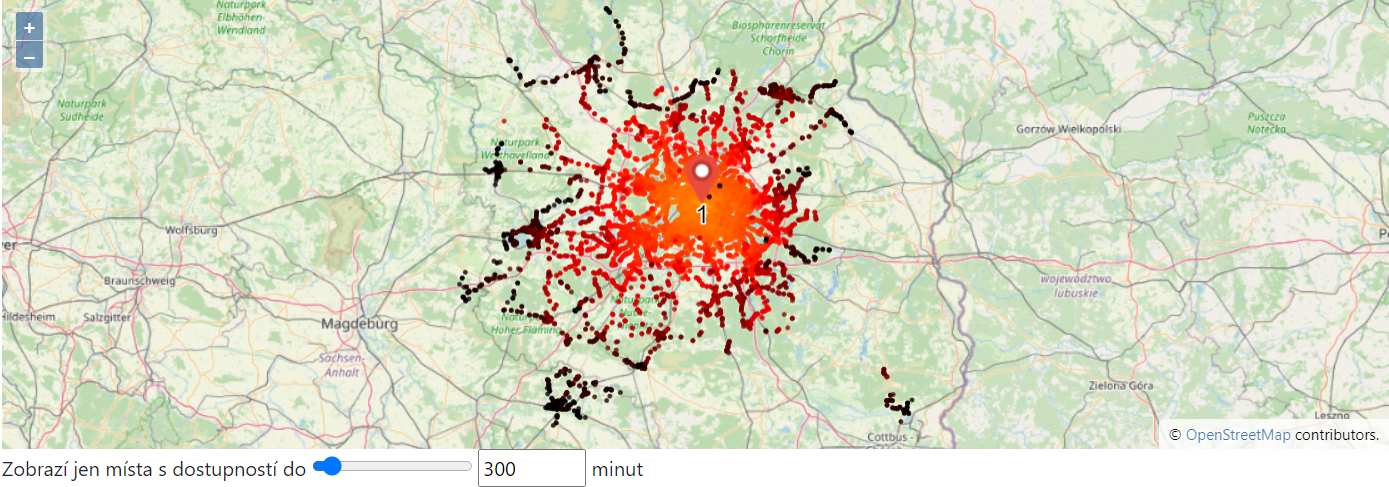
\includegraphics[width=\textwidth]{../img/Nemecko-Berlin.png}
    \caption{Vizualizaci dostupnosti do 300 minut v~okolí Berlínu.}
    \label{fig:Nemecko-Berlin}
\end{figure}

\chapter*{Závěr}
\addcontentsline{toc}{chapter}{Závěr}

V~této práci jsme chtěli ohodnotit všechna místa podle dostupnosti veřejnou dopravou. To se nám v~podstatě podařilo. Jediným možným nedostatkem je to, že počítáme dostupnost z~míst zadaných uživatelem na všechna ostatní místa, ale neřešíme již dostupnost v~opačném směru. Možné řešení tohoto problému jsme však navrhovali v~sekci~\ref{raptor-inverze}.
Dostupnost jsme chtěli vizualizovat na všech místech. Nám se podařilo vizualizovat dostupnost pro body v~daném rozlišení. Pro větší území potřebujeme počítat dostupnost v~bodech ve větším rozlišení. Avšak předvýpočet spojený s~vyhodnocováním bodů může být pro velké rozlišení neprakticky dlouhý.
Jak jsme plánovali, výsledná aplikace je schopna pracovat s~jízdními řády z~různých lokalit. Při práci s~velkými daty jízdních řádů, jako poskytuje například Německo, však začínáme mít výkonnostní problémy. %pridat ref?


Výsledkem této práce je knihovna a~webová aplikace. Knihovnu lze využívat nezávisle na webové aplikaci a~nejspíše by se dala použít i~pro řešení jiných problémů, které by vyžadovaly ohodnocení dostupnosti veřejnou dopravou. Webová aplikace pracuje s~interaktivní mapou. Společně zpřístupňují naši knihovnu běžným uživatelům a~usnadňují orientaci ve výsledných dostupnostech. 


Vedle optimalizací a~nápadů na zlepšení, zmíněných v~předchozích kapitolách, bychom v~budoucnu mohli rozšířit funkcionalitu naší aplikace.
Naše aplikace by ve spojení s~cenovou mapou\footnote{Pro Prahu je cenová mapa dostupná na adrese \url{https://app.iprpraha.cz/apl/app/cenova-mapa/}} mohla vypočítávat poměr dostupnosti a~ceny pozemku.
Pokud bychom měli přístup k~právě pronajímaným či prodávaným nemovitostem, mohli bychom je seřadit dle dostupnosti nebo bychom mohli opět určovat poměr dostupnosti a~ceny.
Aplikaci bychom mohli rozšiřovat i~jiným směrem.
Některé lidi by vedle dostupnosti veřejnou dopravou mohlo zajímat, v~jaké vzdálenosti od daného místa jsou nemocnice, školy, obchody a~další často navštěvované budovy. Takovéto budovy bychom mohli vyhledat například pomocí dotazů v~jazyce SPARQL (SPARQL Protocol and RDF Query Language) na stránce wikidat\footnote{Wikidata dotazy lze psát na adrese \url{https://query.wikidata.org/}}.


%%% Seznam použité literatury
%%% Seznam použité literatury (bibliografie)
%%%
%%% Pro vytváření bibliografie používáme bibTeX. Ten zpracovává
%%% citace v textu (např. makro \cite{...}) a vyhledává k nim literaturu
%%% v souboru literatura.bib.
%%%
%%% Příkaz \bibliographystyle určuje, jakým stylem budou citovány odkazy
%%% v textu. V závorce je název zvoleného souboru .bst. Styly plainnat
%%% a unsrt jsou standardní součástí latexových distribucí. Styl czplainnat
%%% je dodáván s touto šablonou a bibTeX ho hledá v aktuálním adresáři.

\bibliographystyle{czplainnat}    %% Autor (rok) s českými spojkami
% \bibliographystyle{plainnat}    %% Autor (rok) s anglickými spojkami
% \bibliographystyle{unsrt}       %% [číslo]

\renewcommand{\bibname}{Seznam použité literatury}

%%% Vytvoření seznamu literatury. Pozor, pokud jste necitovali ani jednu
%%% položku, seznam se automaticky vynechá.

\bibliography{literatura}

%%% Kdybyste chtěli bibliografii vytvářet ručně (bez bibTeXu), lze to udělat
%%% následovně. V takovém případě se řiďte normou ISO 690 a zvyklostmi v oboru.

% \begin{thebibliography}{99}
%
% \bibitem{lamport94}
%   {\sc Lamport,} Leslie.
%   \emph{\LaTeX: A Document Preparation System}.
%   2. vydání.
%   Massachusetts: Addison Wesley, 1994.
%   ISBN 0-201-52983-1.
%
% \end{thebibliography}


%%% Obrázky v bakalářské práci
%%% (pokud jich je malé množství, obvykle není třeba seznam uvádět)
\listoffigures

%%% Tabulky v bakalářské práci (opět nemusí být nutné uvádět)
%%% U matematických prací může být lepší přemístit seznam tabulek na začátek práce.
%\listoftables

%%% Použité zkratky v bakalářské práci (opět nemusí být nutné uvádět)
%%% U matematických prací může být lepší přemístit seznam zkratek na začátek práce.
%\chapwithtoc{Seznam použitých zkratek}

%%% Přílohy k bakalářské práci, existují-li. Každá příloha musí být alespoň jednou
%%% odkazována z vlastního textu práce. Přílohy se číslují.
%%%
%%% Do tištěné verze se spíše hodí přílohy, které lze číst a prohlížet (dodatečné
%%% tabulky a grafy, různé textové doplňky, ukázky výstupů z počítačových programů,
%%% apod.). Do elektronické verze se hodí přílohy, které budou spíše používány
%%% v elektronické podobě než čteny (zdrojové kódy programů, datové soubory,
%%% interaktivní grafy apod.). Elektronické přílohy se nahrávají do SISu a lze
%%% je také do práce vložit na CD/DVD. Povolené formáty souborů specifikuje
%%% opatření rektora č. 72/2017.
\appendix
\chapter{Přílohy}

%sekce pro kod programu ? - Elektronicka priloha

\section{Dokumentace}

\subsubsection{Uživatelská dokumentace}

Uživatelská dokumentace je součástí webové stránky. Konkrétně je popsaná na úvodní stránce. Pro jednodušší přístup přikládáme uživatelskou dokumentaci do elektronické přílohy této práce.

\subsubsection{Programátorská dokumentace}

Programátorská dokumentace je obecně popsaná v~kapitole~\ref{kapitola-Implementace}. Dokumentace kódu je vytvořena pomocí XML komentářů. Samotný kód přikládáme v~elektronické příloze.


\subsection{Instalace}

\subsubsection{Prerekvizity}

Ke spuštění či překladu aplikace potřebujeme platformu .NET~5.0, která je k~dispozici na stránkách Microsoftu\footnote{Ke stažení na stránce \url{https://dotnet.microsoft.com/en-us/download/dotnet/5.0}}.

Instalace platformy .NET~5.0 nám zpřístupní příkaz \textbf{dotnet}, pomocí kterého aplikaci spustíme. Alternativně můžeme ke spuštění využít nástroje poskytované prostředím \textbf{Visual Studia}.

\subsubsection{Spuštění}

Aplikaci přeložíme zavoláním příkazu \textbf{dotnet build} z~adresáře obsahujícího aplikaci.

Příkaz \textbf{dotnet run -{}-project src/Web/Web.csproj} použijeme ke spuštění naší webové aplikace.

Pro ověření funkčnosti aplikace můžeme spustit \textbf{Unit Testy} pomocí příkazu \textbf{dotnet test}.


\subsection{Konfigurační soubor}

% popsat ze je urcen pro spravce webove aplikace, ktery ho meni

\subsubsection{GTFS data}

Konstanta \textbf{ShouldUpdate} určuje, zdali chceme při spuštění aplikace data aktualizovat, viz popis třídy \textbf{DataUpdater} v~sekci~\ref{trida-DataUpdater}. Při aktualizaci dojde ke stažení dat a~k~jejich deserializaci. Pokud data neaktualizujeme, serializujeme dříve uložená data.

URL pro stažení dat specifikujeme konstantou \textbf{GTFSSourceURI}. Aktuálně podporujeme jen data archivovaná ve formátu zip.

% mohla by byt podsekce `zpracovani dat`
Data stahujeme do složky určené konstantou \textbf{PathToGTFSFolder} a~cestu k~serializaci určuje konstanta \textbf{GTFSSerializationPath}.

Platnost dat závisí na konkrétním zprostředkovateli a~dá se nastavit skrze konstantu \textbf{ValidityInDays}.

UTC offset pro časy jízdních řádů, které uchováváme na serveru, lze nastavit konstantou \textbf{UTCOffset}.

\subsubsection{Přestupy}

Generování přestupů popisujeme v~sekci~\ref{generovani-prestupu}.

Konstantu \textbf{MaxTransferDistanceInMeters} používáme pro omezení vzdálenosti během generování přestupů.

Konstantu \textbf{WalkingSpeedInMetersPerSec} určuje průměrnou rychlost chůze. Používáme ji k~odhadu času potřebného pro přestup.

\subsubsection{Sousední zastávky}

Sousední zastávky detailně popisujeme v~sekci~\ref{class-NearestStops}.

Konstantu \textbf{WalkingSpeedInMetersPerSec} používáme také pro odhad času potřebného k~příchodu z~nějakého místa na zastávky v~okolí.

Konstanta \textbf{NearestStopsDistanceInMeters} omezuje vzdálenost, ve které hledáme z~daného místa sousední zastávky.

\subsubsection{Vizualizace bodů}

Konstanta \textbf{VisualisedRasterPointsResolution} určuje rozlišení, pro které vizualizujeme dostupnost v~bodech, viz sekce~\ref{optim-body}.

\openright
\end{document}
